% !TEX program = lualatex
\documentclass[a4paper]{article}
\usepackage{svg}
\usepackage{amsthm}
\usepackage{fontspec}
\setmainfont{Latin Modern Roman}
\usepackage[vietnamese]{babel}
\usepackage{pdflscape}
\usepackage{subcaption} % Thêm vào preamble của main.tex
\usepackage{rotating}
\usepackage{a4wide,amssymb,epsfig,latexsym,multicol,array,hhline,fancyhdr}
\usepackage{minted}
\usepackage{booktabs} % Cho bảng đẹp
\usepackage{longtable} % Cho bảng dài
\usepackage{placeins}
\usepackage{capt-of}
\usepackage{tabularx} % Cho bảng có cột co giãn
\usepackage{caption}
\usepackage{subcaption}
\usepackage{tabularx}
\usepackage{booktabs}
\usepackage{amsmath}
\usepackage{float}
\usepackage{lastpage} 
% \usepackage[lined,boxed,commentsnumbered]{algorithm2e}
\usepackage{enumerate}
\usepackage{color}
\usepackage{graphicx}					% Standard graphics package
\usepackage{array}
\usepackage{tabularx, caption}
\usepackage{multirow}
\usepackage[framemethod=tikz]{mdframed}% For highlighting paragraph backgrounds
\usepackage{multicol}
\usepackage{rotating}
\usepackage{graphics}
\usepackage{wrapfig}
\usepackage{geometry}
\usepackage{setspace}
\usepackage{epsfig}
\usepackage{tikz}
\usepackage{pgfplots}
\pgfplotsset{compat=newest}
\usepackage{listings}
\usetikzlibrary{arrows,arrows.meta,snakes,backgrounds,calc}
\usepackage{hyperref}
\usepackage{minted}
\usepackage{indentfirst}
\usepackage{cases} 
\usepackage{listings}
\usepackage{algorithm}
\usepackage{algpseudocode}
% \usepackage[english]{babel}
\renewcommand{\baselinestretch}{1.5}
\usepackage[table]{xcolor}
\usepackage[most]{tcolorbox}
\renewcommand{\figurename}{Hình}
\definecolor{termBG}{HTML}{0C1C23}
\definecolor{termWhite}{HTML}{F8F8F2}

\lstset{
    language=C++,
    basicstyle=\ttfamily\footnotesize,
    numbers=left,
    numberstyle=\tiny,
    stepnumber=1,
    numbersep=5pt,
    backgroundcolor=\color{gray!10},
    keywordstyle=\color{blue}\bfseries,
    commentstyle=\color{green!50!black},
    stringstyle=\color{red},
    frame=single,
    breaklines=true,
}

\usepackage[most]{tcolorbox}
\newtcbox{\code}{on line, 
    arc=2pt,                % Độ bo tròn góc
    colback=gray!20,        % Màu nền (xám nhạt)
    colframe=gray!20,       % Viền cùng màu nền
    boxrule=0pt,            % Không độ dày viền
    boxsep=0pt, left=2pt, right=2pt, top=2pt, bottom=2pt, % Khoảng cách đệm
    fontupper=\ttfamily     % Font chữ kiểu code
}

\newtcolorbox{softbox}{
    colback=black!3,        % Màu nền: Xám rất nhạt (3% đen)
    colframe=black!3,       % Màu viền: Trùng màu nền (để không thấy viền)
    arc=8pt,                % Độ bo tròn góc
    boxrule=0pt,            % Độ dày viền = 0
    left=10pt, right=10pt, top=8pt, bottom=8pt, % Khoảng cách lề bên trong
    fontupper=\itshape\color{black!80} % Font chữ: Nghiêng và màu xám đậm (80% đen)
}

\definecolor{codegreen}{rgb}{0,0.6,0}
\definecolor{codegray}{rgb}{0.5,0.5,0.5}
\definecolor{codepurple}{rgb}{0.58,0,0.82}
\definecolor{backcolour}{rgb}{0.95,0.95,0.92}

\definecolor{termBG}{HTML}{0C1C23}    % Màu nền xanh đen đậm
\definecolor{termRed}{HTML}{FF5555}   % Màu đỏ
\definecolor{termYellow}{HTML}{F1FA8C}% Màu vàng
\definecolor{termWhite}{HTML}{F8F8F2} % Màu chữ trắng sáng
\definecolor{termGray}{HTML}{A9B7C6}  % Màu xám nhạt (nếu cần)

\newtcolorbox{TerminalBox}{
    colback=termBG,       
    coltext=termWhite,    
    boxrule=0pt,          
    arc=3pt,              
    left=4pt, right=4pt, top=4pt, bottom=4pt, % Giảm lề đệm xuống 4pt cho gọn
    % QUAN TRỌNG: Dùng \tiny để chữ siêu nhỏ
    fontupper=\ttfamily\scriptsize\linespread{1.0}\selectfont, 
    enhanced
}

% Lệnh tắt để tô màu cho nhanh
\newcommand{\cred}[1]{\textcolor{termRed}{#1}}
\newcommand{\cyellow}[1]{\textcolor{termYellow}{#1}}

% Cấu hình style cho C++
\lstdefinestyle{mystyle}{
    backgroundcolor=\color{backcolour},   
    commentstyle=\color{codegreen},
    keywordstyle=\color{magenta},
    numberstyle=\tiny\color{codegray},
    stringstyle=\color{codepurple},
    basicstyle=\ttfamily\footnotesize, % Font chữ kiểu máy đánh chữ, kích thước nhỏ
    breakatwhitespace=false,         
    breaklines=true,                 % Tự động xuống dòng nếu quá dài
    captionpos=b,                    
    keepspaces=true,                 
    numbers=left,                    % Hiển thị số dòng bên trái
    numbersep=5pt,                  
    showspaces=false,                
    showstringspaces=false,
    showtabs=false,                  
    tabsize=2,                       % Độ rộng tab = 2 spaces
    language=C++                     % Ngôn ngữ C++
}

\lstset{style=mystyle}
\lstdefinestyle{ciscoTerminal}{style=mystyle}
% ---------------------------------

\usepackage{hyperref}
\hypersetup{
    colorlinks=true,
    linkcolor=black,      % Màu link nội bộ (mục lục, cross-reference)
    citecolor=red,        % ← Màu citation (references) - ĐỔI THÀNH ĐỎ
    urlcolor=blue,        % Màu URL
    filecolor=magenta     % Màu link file
}

%%%%%%%%
\usepackage{longtable}
\usepackage[shortlabels]{enumitem}

\setlength{\headheight}{40pt}
\setlength{\footskip}{36pt}
\pagestyle{fancy}
\fancyhead{} % clear all header fields
\fancyhead[L]{
 \begin{tabular}{rl}
    
\includegraphics[width=8mm, height=8mm]{images/khtn.png}&
	\begin{tabular}{l}
		\textbf{\bf \ttfamily Ho Chi Minh University of Science - VNUHCM}\\
		\textbf{\bf \ttfamily Faculty of Information Technology}
	\end{tabular}
 \end{tabular}
}
\fancyhead[R]{
	\begin{tabular}{l}
		\tiny \bf \\
		\tiny \bf 
	\end{tabular}  }
\fancyfoot{} % clear all footer fields
\makeatletter
\newcommand{\footerfootnotetext}{\@empty}
\newcommand{\footerfootnote}[1]{%
    \refstepcounter{footnote}%
    \textsuperscript{\thefootnote}%
    \g@addto@macro\footerfootnotetext{\textsuperscript{\thefootnote} #1\space}%
}
\newcommand{\printfooterfootnote}{%
    \ifx\footerfootnotetext\@empty\else
        \footerfootnotetext\\
    \fi
}
\AddToHook{shipout/after}{\global\let\footerfootnotetext\@empty}
\makeatother
\fancyfoot[L]{\scriptsize \ttfamily \parbox[b]{0.78\textwidth}{\printfooterfootnote Applied Mathematics in Statistics}}
\fancyfoot[R]{\scriptsize \ttfamily Page {\thepage}}
\renewcommand{\headrulewidth}{0.3pt}
\renewcommand{\footrulewidth}{0.3pt}


%%%
\setcounter{secnumdepth}{4}
\setcounter{tocdepth}{3}
\makeatletter
\newcounter {subsubsubsection}[subsubsection]
\renewcommand\thesubsubsubsection{\thesubsubsection .\@alph\c@subsubsubsection}
\newcommand\subsubsubsection{\@startsection{subsubsubsection}{4}{\z@}%
                                    {-3.25ex\@plus -1ex \@minus -.2ex}%
                                    {1.5ex \@plus .2ex}%
                                    {\normalfont\normalsize\bfseries}}
\newcommand*\l@subsubsubsection{\@dottedtocline{3}{10.0em}{4.1em}}
\newcommand*{\subsubsubsectionmark}[1]{}
\makeatother

\definecolor{dkgreen}{rgb}{0,0.6,0}
\definecolor{gray}{rgb}{0.5,0.5,0.5}
\definecolor{mauve}{rgb}{0.58,0,0.82}

\lstset{frame=tb,
	language=Matlab,
	aboveskip=3mm,
	belowskip=3mm,
	showstringspaces=false,
	columns=flexible,
	basicstyle={\small\ttfamily},
	numbers=none,
	numberstyle=\tiny\color{gray},
	keywordstyle=\color{blue},
	commentstyle=\color{dkgreen},
	stringstyle=\color{mauve},
	breaklines=true,
	breakatwhitespace=true,
	tabsize=3,
	numbers=left,
	stepnumber=1,
	numbersep=1pt,    
	firstnumber=1,
	numberfirstline=true
}

%  MÀU SẮC
\definecolor{primaryblue}{RGB}{0, 70, 127}
\definecolor{accentblue}{RGB}{52, 144, 220}
\definecolor{lightgray}{RGB}{245, 247, 250}
\definecolor{codegray}{RGB}{240, 240, 240}
\definecolor{darkgray}{RGB}{80, 80, 80}
\definecolor{successgreen}{RGB}{40, 167, 69}
\definecolor{warnorange}{RGB}{255, 140, 0}

%  HỘP LÝ THUYẾT
\tcbuselibrary{theorems, skins, breakable}
\tcbset{
    defstyle/.style={
        enhanced, breakable,
        colback=lightgray, colframe=primaryblue,
        fonttitle=\bfseries,
        attach boxed title to top left={yshift=-2mm, xshift=4mm},
        boxed title style={colback=primaryblue, colframe=primaryblue},
        top=4mm
    },
    thmstyle/.style={
        enhanced, breakable,
        colback=blue!5!white, colframe=accentblue,
        fonttitle=\bfseries,
        attach boxed title to top left={yshift=-2mm, xshift=4mm},
        boxed title style={colback=accentblue, colframe=accentblue},
        top=4mm
    },
    notestyle/.style={
        enhanced, breakable,
        colback=yellow!10!white, colframe=warnorange,
        fonttitle=\bfseries\color{warnorange},
        left=2mm
    }
}
\newtcbtheorem[number within=section]{mydef}{Định nghĩa}{defstyle}{def}
\newtcbtheorem[number within=section]{mythm}{Định lý}{thmstyle}{thm}
\newtcbtheorem[number within=section]{mylem}{Bổ đề}{thmstyle}{lem}
\newtcbtheorem[number within=section]{myprop}{Mệnh đề}{thmstyle}{prop}
\newtcbtheorem[number within=section]{mycor}{Hệ quả}{defstyle}{cor}
\newenvironment{note}[1][Ghi chú]{%
    \begin{tcolorbox}[notestyle, title=#1]}{%
    \end{tcolorbox}}

%  TOÁN HỌC
\newcommand{\R}{\mathbb{R}}
\newcommand{\C}{\mathbb{C}}
\newcommand{\norm}[1]{\left\lVert#1\right\rVert}
\newcommand{\inner}[2]{\langle #1,\, #2 \rangle}
\newcommand{\E}{\mathbb{E}}
\newcommand{\proj}[2]{\operatorname{proj}_{#2}\!\left(#1\right)}
\providecommand{\coloneqq}{\mathrel{\mathop:}=}
\newcommand{\rank}{\operatorname{rank}}
\newcommand{\tr}{\operatorname{tr}}
\newcommand{\col}{\operatorname{col}}
\newcommand{\spann}{\operatorname{span}}
\newcommand{\mat}[1]{\mathbf{#1}}

\begin{document}

\begin{titlepage}
\begin{center}
VIETNAM NATIONAL UNIVERSITY HO CHI MINH CITY\\
HO CHI MINH CITY UNIVERSITY OF SCIENCE \\
FACULTY OF INFORMATION TECHNOLOGY
\end{center}

\vspace{0.7cm}

\begin{figure}[h!]
\begin{center}

\includegraphics[width=5cm]{images/khtn.png}
\end{center}
\end{figure}

\vspace{0.5cm}


\begin{center}
\begin{tabular}{c}
\multicolumn{1}{c}{\textbf{{\normalsize DEPARTMENT OF COMPUTER SCIENCE}}}\\
~~\\
\hline
\\
\multicolumn{1}{c}{\textbf{{\Large REPORT OF PROJECT 1}}}\\  % ← Đổi từ {l} thành {c}
\\
\textbf{{\Large Project: Data Fitting and Ordinary Least Squares Method}}\\
\\
\hline
\end{tabular}
\end{center}

\vspace{0.5cm}

\begin{table}[h]
\begin{tabular}{rrll}
\hspace{4.5cm} & \textbf{Lecturer:} & ThS. Võ Nam Thục Đoan\\
\hspace{4.5cm} &  & ThS. Lê Nhựt Nam\\
\hspace{4.5cm} & \textbf{Leader:} & Khang Phuc Nguyen & 24120068\\
\hspace{4.5cm} & Members: & Nghia Trong Hoang & 24120103\\
\hspace{4.5cm} &  & Nhat Hoang Mai & 24120109 \\
\hspace{4.5cm} &  & Nhat Hoang Nguyen & 24120110 \\
\hspace{4.5cm} &  & Long Nhat Phung Vo & 24120088\\

\end{tabular}
\end{table}

\vspace{1.2cm}

\begin{center} {\footnotesize Ho Chi Minh City, 4/2026}
\end{center}
\end{titlepage}
%\thispagestyle{empty}


\thispagestyle{empty}

\newpage
\renewcommand{\contentsname}{Table of Contents}
\renewcommand{\tablename}{Table}
\renewcommand{\figurename}{Figure}
\renewcommand{\refname}{References}
\renewcommand{\listfigurename}{List of Figures}
\renewcommand{\listtablename}{List of Tables}

\tableofcontents

\newpage

\renewcommand{\arraystretch}{1.3} % Adjust row height
\setcounter{page}{1}
\vspace{1cm}

\section{Bài Toán Data Fitting và Phương Pháp OLS}

\subsection{Phát Biểu Bài Toán Data Fitting Tổng Quát}
Bài toán Data Fitting đã có nền tảng toán học và lịch sử từ lâu đời, nó luôn đi chung với sự phát triển của phương pháp \textbf{Bình Phương Tối Thiểu (OLS)}. Bài toán được hình thành được đặt ra không chỉ để thỏa mãn niềm đam mê toán học của các nhà nghiên cứu mà nó còn có mục đích rất thực tiễn trong các ngành liên quan về thiên văn học và trắc địa vào cuối thế kỷ 18 và đầu thế kỷ 19.
\subsubsection{Đặt vấn đề}
Vào những năm 1790, để có thể thiết lập ra hệ mét \footerfootnote{Hệ mét là hệ thống đo lường thập phân được thống nhất rộng rãi trên quốc tế. Dù có nhiều biến thể của hệ thống số liệu nổi lên vào cuối thế kỷ XIX và đầu thế kỷ XX, thuật ngữ này thường được dùng như một từ đồng nghĩa là "SI" hoặc "Hệ thống đơn vị Quốc Tế"} thì ông đã phải đo đạc chính xác chiều dài \textbf{cung kinh tuyến} từ cực Bắc đến Xích đạo đi qua Paris \cite{stigler1996}. Họ đã không trực tiếp mà họ đo một đoạn cung kinh tuyến, cụ thể là đoạn từ \textit{Runkirk} đến \textit{Barcelona}, rồi dùng mô hình toán học để suy ra độ đài \textbf{một phần tư kinh tuyến Trái Đất}.

Do đó ta có thể thấy rằng, bài toán \textbf{Data Fitting} đã xuất hiện từ rất lâu và nó đã trở thành một trong những bài toán kinh điển trong Toán học và là nền tảng cho các mô hình học máy sau này. Cụ thể hơn, ta có một tập dữ liệu quan sát được
và muốn tìm một hàm số mô tả mối quan hệ giữa đầu vào và đầu ra. Bài toán này
được gọi chung là \textbf{data fitting} (khớp dữ liệu).

\begin{mydef}{Bài toán Data Fitting tổng quát}{}
Cho tập dữ liệu $\mathcal{D} = \{(\mat{x}_i, y_i)\}_{i=1}^n$ với
$\mat{x}_i \in \R^p$, $y_i \in \R$. Bài toán data fitting là tìm hàm
$f : \R^p \to \R$ trong một lớp hàm cho trước $\mathcal{F}$ sao cho
$f$ xấp xỉ tốt nhất ánh xạ từ $\mat{x}_i$ đến $y_i$ theo một tiêu chí tối ưu:
\[
    \hat{f} = \arg\min_{f \in \mathcal{F}} \mathcal{L}(f;\, \mathcal{D}),
\]
trong đó $\mathcal{L}$ là hàm mất mát (\textit{loss function}) đo mức độ sai lệch
giữa dự đoán của mô hình và giá trị thực.
\end{mydef}

\subsubsection{Mô hình hồi quy tuyến tính}
Mô hình hồi quy tuyến tính là nền tảng cốt lõi trong toán học thống kê, nó có lịch sử phát triển gắn với bài toán Data Fitting và phương pháp bình phương tối thiểu. Mục tiêu của mô hình là có thể \textit{ước lượng các tham số chưa biết thông qua các dữ liệu thực nghiệm đã quan sát được} \cite{plackett1972}. Trong mô hình này, các quan sát được biểu diễn dưới dạng một \textbf{tổ hợp tuyến tính} của các biến đã biết và các \textbf{tham số ẩn}.  

Giả sử ta có một chuỗi các quan sát $y_i$ phụ thuộc vào một mô hình tuyến tính $\alpha + \beta x_i$ ($i = 1, ...,n)$. Bài toán đặt ra là làm sao ta có thể ước lượng các giá trị $\hat{\alpha}$ và $\hat{\beta}$ cho các tham số $\alpha$ và $\beta$ để có thể phù hợp với bộ dữ liệu quan sát được một cách tốt nhất và ít chi phí nhất \cite{plackett1972}. Tổng quát bài toán, thì phần lớn ta sẽ có thể viết mô hình dưới dạng $Y = M\beta + \theta$ và cụ thể hơn $\mathcal{F}$ là tập
các hàm tuyến tính theo tham số~\cite{strang2023}. Khi đó, giả thiết:
\[
    y_i = \beta_0 + \beta_1 x_{i1} + \beta_2 x_{i2} + \cdots + \beta_p x_{ip}
        + \varepsilon_i
        = \mat{x}_i^T \boldsymbol{\beta} + \varepsilon_i,
\]
với $\boldsymbol{\beta} = (\beta_0, \beta_1, \ldots, \beta_p)^T \in \R^{p+1}$
là vector tham số cần ước lượng và $\varepsilon_i$ là nhiễu ngẫu nhiên (sai số
mô hình).

Đặt ma trận thiết kế (\textit{design matrix})
$\mat{X} \in \R^{n \times (p+1)}$ trong đó hàng thứ $i$ là
$(1,\, x_{i1},\, \ldots,\, x_{ip})$ (cột đầu tiên toàn số 1 ứng với hệ số tự
do $\beta_0$). Khi đó toàn bộ hệ có thể viết gọn:

\begin{equation}
    \mat{y} = \mat{X}\boldsymbol{\beta} + \boldsymbol{\varepsilon},
    \qquad \mat{y} \in \R^n,\;
           \mat{X} \in \R^{n \times (p+1)},\;
           \boldsymbol{\varepsilon} \in \R^n.
    \label{eq:linear_model}
\end{equation}

\begin{figure}[H]
\centering
\begin{tikzpicture}[>=Stealth, scale=1.0,
    node/.style={draw=primaryblue, rounded corners=4pt,
                 fill=lightgray, minimum width=2.2cm,
                 minimum height=0.85cm, font=\small}]
  % Nodes
  \node[node] (X)    at (0,0)   {$\mat{X} \in \R^{n\times(p+1)}$};
  \node[node] (beta) at (4.2,0) {$\boldsymbol{\beta} \in \R^{p+1}$};
  \node[node] (Xb)   at (8.4,0) {$\mat{X}\boldsymbol{\beta} \in \R^n$};
  \node[node] (eps)  at (8.4,-1.6) {$\boldsymbol{\varepsilon} \in \R^n$};
  \node[node, fill=blue!8!white, draw=accentblue]
             (y)     at (12.0,-0.75) {$\mat{y} \in \R^n$};

  % Arrows
  \draw[->, thick, primaryblue] (X)   -- node[above,font=\footnotesize]{nhân} (beta);
  \draw[->, thick, primaryblue] (beta)-- (Xb);
  \draw[->, thick, accentblue]  (Xb)  -- node[right,font=\footnotesize,xshift=2pt]{$+$} (y);
  \draw[->, thick, warnorange]  (eps) -- node[right,font=\footnotesize]{nhiễu} (y);
\end{tikzpicture}
\caption{Cấu trúc mô hình hồi quy tuyến tính dạng ma trận:
$\mat{y} = \mat{X}\boldsymbol{\beta} + \boldsymbol{\varepsilon}$.
Dữ liệu quan sát $\mat{y}$ được phân tích thành thành phần \textit{tín hiệu}
$\mat{X}\boldsymbol{\beta}$ (xanh) và thành phần \textit{nhiễu}
$\boldsymbol{\varepsilon}$ (cam).}
\label{fig:linear_model}
\end{figure}

% ============================================================
\subsection{Các Giả Thiết Gauss–Markov}

Trong quá trình phát triển của phương pháp OLS, ban đầu Gauss đã đề xuất ra một cách chứng minh dựa trên nền tảng xác suất và phân phối. Nhưng mà cách chứng minh này lại có hạn chế là ép đặt phân phối sai số ban đầu phải tuân theo phân phối chuẩn hình chuông. Sau đó chính bản thân ông đã nhận ra sai lầm của mình mà từ đó đề xuất ra một cách chứng minh khác đó là Gauss-Markov dựa trên các giả thiết sau:

Để ước lượng OLS có các tính chất thống kê tốt, mô hình tuyến tính~\eqref{eq:linear_model}
cần thỏa mãn năm giả thiết Gauss--Markov sau~\cite{wooldridge2013,greene2012}. Các giả thiết này xác định khuôn khổ
mà trong đó OLS được đảm bảo là ước lượng tốt nhất.

\begin{mydef}{Các giả thiết Gauss--Markov (GM1–GM5)}{}
\begin{enumerate}[label=\textbf{\arabic*.}, leftmargin=2.5cm, noitemsep]
    \item \textbf{Tuyến tính:} $\mat{y} = \mat{X}\boldsymbol{\beta} + \boldsymbol{\varepsilon}$.
          Mô hình tuyến tính theo tham số $\boldsymbol{\beta}$; cho phép áp dụng
          đại số tuyến tính để giải bài toán tối ưu.

    \item \textbf{Không hoàn hảo đa cộng tuyến:} $\rank(\mat{X}) = p + 1$,
          tức các cột của $\mat{X}$ độc lập tuyến tính và $\mat{X}^T\mat{X}$ khả nghịch.
          Nếu vi phạm, nghiệm OLS không xác định duy nhất.

    \item \textbf{Ngoại sinh (zero conditional mean):}
          $\E[\boldsymbol{\varepsilon} \mid \mat{X}] = \mat{0}$,
          tức $\E[\varepsilon_i \mid \mat{x}_i] = 0$ với mọi $i$.
          Đảm bảo không có biến quan trọng bị bỏ sót có tương quan với $\mat{X}$.

    \item \textbf{Đồng phương sai (homoscedasticity):}
          $\mathrm{Var}(\boldsymbol{\varepsilon} \mid \mat{X}) = \sigma^2\mat{I}_n$,
          tức $\mathrm{Var}(\varepsilon_i) = \sigma^2$ và
          $\mathrm{Cov}(\varepsilon_i, \varepsilon_j) = 0$ với $i \neq j$.
          Nếu vi phạm (heteroscedasticity), sai số chuẩn bị lệch.

    \item \textbf{Phần dư chuẩn (normality):}
          $\boldsymbol{\varepsilon} \mid \mat{X} \sim \mathcal{N}(\mat{0},\, \sigma^2\mat{I}_n)$.
          \emph{Điều kiện bổ sung — cần cho kiểm định $t$ và $F$ trong mẫu nhỏ;
          với mẫu lớn có thể nới lỏng nhờ định lý giới hạn trung tâm.}
\end{enumerate}
\end{mydef}

\begin{note}
Giả thiết $1–4$ đủ để đảm bảo OLS là \textbf{BLUE} (Best Linear Unbiased Estimator)
theo Định lý Gauss--Markov (xem mục~\ref{subsec:blue} bên dưới).
Giả thiết $5$ chỉ cần thiết khi thực hiện kiểm định giả thuyết và xây dựng khoảng tin cậy.
\end{note}

% ============================================================
\subsection{Hàm Mất Mát RSS và Chứng Minh Nghiệm OLS}
Hàm mất mát Residual Sum of Squares được gọi là tổng bình phương các sai số, là mục tiêu cốt lõi khi các nhà toán học làm việc với bài toán Data Fitting, họ sẽ cố gắng \textbf{tối thiểu hóa} hàm mất này để có thể tạo ra mô hình tốt nhất cho tập dữ liệu mà họ có, điều này rất phổ biến trong phương pháp bình phương tối thiểu và hồi quy.
\subsubsection{Hàm mất mát RSS}

Vào khoảng năm 1805, nhà toán học Andrien-Marie Legendre đã xây dựng một hệ phương trình tuyến tính cho các quan sát mà ông có được, trong đó mỗi phương trình của hệ có một sai số $E$. Hàm mất RSS được ông ký hiệu là $S$ đại diện cho tổng bình phương của tất cả các sai số này với $S = E^2 + E'^2 + E''^2 + ...$ \cite{plackett1972}
\begin{mydef}{Residual Sum of Squares (RSS)}{}
Hàm mất mát của phương pháp Ordinary Least Squares (OLS) là tổng bình phương
phần dư (\textit{Residual Sum of Squares}):
\[
    \mathrm{RSS}(\boldsymbol{\beta})
    = \norm{\mat{y} - \mat{X}\boldsymbol{\beta}}_2^2
    = \sum_{i=1}^n \bigl(y_i - \mat{x}_i^T\boldsymbol{\beta}\bigr)^2.
\]
OLS tìm $\hat{\boldsymbol{\beta}}$ tối thiểu hóa $\mathrm{RSS}(\boldsymbol{\beta})$.
\end{mydef}

\begin{note}[Ý nghĩa hình học]
RSS đo tổng bình phương khoảng cách từ các điểm quan sát $y_i$ đến các giá trị
dự đoán $\hat{y}_i = \mat{x}_i^T\boldsymbol{\beta}$ của mô hình. OLS tìm
hyperplane tốt nhất theo nghĩa cực tiểu hóa tổng khoảng cách vuông góc theo
chiều $y$.
\end{note}

Với sự ra đời của RSS thì bài toán OLS đã trở nên rõ ràng hơn, nó đã cung cấp một công cụ mạnh mẽ để ước lượng các tham số của mô hình hồi quy tuyến tính, từ đó giúp các nhà nghiên cứu có thể hiểu rõ hơn về mối quan hệ giữa các biến và đưa ra dự đoán chính xác hơn dựa trên dữ liệu quan sát được. \textit{(1) Tạo ra sự cân bằng và triệt tiêu sai số cực đoan}. Điều này đã được Legendre lập luận và chứng minh rằng hàm bình phương mang lại một sự cân bằng lớn giữa các sai số. Nó đưa ra điểm phạt rất lớn cho các sai số lớn từ đó mà ngăn được các phần tử ngoại lai giúp ta tìm ra trạng thái gần thực tế nhất. \textit{(2) Dễ dàng tính được bằng giải tích}. Khác với hàm giá trị tuyệt đối khác gặp khó khăn lớn trong việc tính toán thì RSS lại mang lại khả năng tính toán vô cùng thuận luận. \textit{(3) Nên tảng xác suất vững chắc}. RSS đã được Gauss chứng minh hoàn hảo thông qua thống kê, ông đã chứng minh rằng nếu các phần dư tuân theo quy luật phân phối chuẩn thì việc cực tiểu hóa hàm mát RSS hoàn toàn tương đương với \textbf{maximum likelihood} \cite{plackett1972}.

\subsubsection{Chứng minh nghiệm OLS (Normal Equations)}
Xuyên suốt lịch sử phát triển, quá trình chứng minh phương pháp Bình Phương tối thiểu là một cuộc hành trình dài từ đầu thế kỷ 19, nó đã đi từ những lập luận đại số thuần túy cho tới nền tảng xác suất và cuối cùng chỉ thật sự được chứng minh tối ưu thông qua hình học trực giao và đại số tuyến tính ma trận hiện đại.

Vào những năm đầu tiên thuở sơ khai của phương pháp, nhà toán học người pháp Legendre đã đề xuất phương pháp OLS kèm theo một cách chứng minh bằng đại số thuần túy, không có yếu tố xác suất đi cùng. Để tìm được giá trị nhỏ nhất của S, ông lấy đạo hàm riêng của S theo từng ẩn số $(x, y, z, ...)$ và cho chúng bằng $0$. Nhờ đó quá trình này đã tạo ra một hệ phương trình tuyến tính mới có nghiệm duy nhất. Tuy nhiên, cách chứng minh này vẫn còn tồn đọng hạn chế là ông chỉ biện minh phương pháp này dựa trên lý luận thực nghiệm rằng bình phương sẽ phạt các sai số lớn, tạo ra \textit{'sự cân bằng'} giữa các quan sát \cite{plackett1972} mà lại không đưa ra được độ chính xác hay sai số của các hệ số tìm được.

Sau đó vào năm 1809, Carl Friedrich Gauss đã đưa ra cách chứng minh của mình được xuất bản bên trong cuốn \textit{Theoria Motus Corporum Coelestium}. Ông đã đưa OLS lên một nền tảng xác suất vững chắc hơn. Gauss sửa dụng nguyên lý \textbf{Hợp lý cực đại} để chứng minh bài toán này. Ông giả sử các sai số đo đạc là các biến ngẫu nhiên độc lập, và từ đó mà đã tìm ra một quy luật phân phối sai số sao cho mà giá trị trung binh cộng chính là giá trị có xác suất xảy ra cao nhất. Điều này đã dẫn tới việc ông tìm ra hàm \textbf{Mật độ xác suất phân phối chuẩn}. Khi mà các sai số tuân theo phân phối chauanr, việc cực đại hóa hàm hợp lý hoàn toàn tương đương về mặt toán học với việc \textbf{cực tiểu hóa tổng bình phương các sai số}.

Và sau Gauss đã có rất nhiều người tham gia vào chứng minh và sửa các hạn chế mà người đi trước mắc phải. Chẳng hạn như sau đó ông Laplace đã đề xuất cách chứng minh để khắc phục hạn chế của Gauss khi ông đang ép buộc sai số phải tuân theo phân phối chuẩn. Laplace đã áp dụng một phiên bản sơ khai của \textbf{Định lý giới hạn trung gian} chứng minh rằng khi số lượng quan sát là rất lớn, thì sự phân phối của tổng hoặc trung bình các sai số sẽ luôn hội tụ về phân phối chuẩn, bất kể phân phối gốc của từng sai số đơn lẻ là gì. Và từ đó mà ông đã chứng minh rằng OLS của Legendre và Gauss là phương pháp mang lại độ chính xác cao nhất cho các tập dữ liệu lớn. Sau này Gauss đã đề xuất cách chứng minh khi không biết quy luật phân phối của sai số ban đầu.

Cuối cùng theo thời gian thì hiện nay ta chứng minh OLS bằng hình học trực giao và đại số ma trận, đây chính là cách được xem là tối ưu, ngắn gọn và đẹp đẽ nhất. Khi nó kết hợp \textbf{Đại số tuyến tính và Phép chiếu trực giao}, là cách tiếp cận bao trùm mọi vấn đề của OLS mà không dùng đến đạo hàm phức tạp.

\begin{mythm}{Nghiệm OLS — Normal Equations}{ols_solution}
Nếu $\mat{X}^T\mat{X}$ khả nghịch (tương đương $\rank(\mat{X}) = p+1$), bài
toán cực tiểu hóa $\mathrm{RSS}(\boldsymbol{\beta})$ có nghiệm duy nhất:
\[
    \hat{\boldsymbol{\beta}}_{\mathrm{OLS}}
    = (\mat{X}^T\mat{X})^{-1}\mat{X}^T\mat{y}.
\]
\end{mythm}

\begin{proof}
Khai triển RSS dưới dạng tích vô hướng để áp dụng giải tích ma trận~\cite{golub2013}:
\begin{align*}
    \mathrm{RSS}(\boldsymbol{\beta})
    &= (\mat{y} - \mat{X}\boldsymbol{\beta})^T
       (\mat{y} - \mat{X}\boldsymbol{\beta}) \\
    &= \mat{y}^T\mat{y}
     - \mat{y}^T\mat{X}\boldsymbol{\beta}
     - \boldsymbol{\beta}^T\mat{X}^T\mat{y}
     + \boldsymbol{\beta}^T\mat{X}^T\mat{X}\boldsymbol{\beta}.
\end{align*}
Vì $\mat{y}^T\mat{X}\boldsymbol{\beta}$ là một số thực (ma trận $1 \times 1$), nó
bằng chuyển vị của chính nó: $\mat{y}^T\mat{X}\boldsymbol{\beta} =
(\mat{y}^T\mat{X}\boldsymbol{\beta})^T = \boldsymbol{\beta}^T\mat{X}^T\mat{y}$.
Do đó:
\[
    \mathrm{RSS}(\boldsymbol{\beta})
    = \mat{y}^T\mat{y}
    - 2\boldsymbol{\beta}^T\mat{X}^T\mat{y}
    + \boldsymbol{\beta}^T\mat{X}^T\mat{X}\boldsymbol{\beta}.
\]

\medskip
\noindent\textbf{Bước 1: Lấy gradient theo $\boldsymbol{\beta}$.}

Áp dụng các công thức đạo hàm ma trận chuẩn:
$\nabla_{\boldsymbol{\beta}}(\mat{a}^T\boldsymbol{\beta}) = \mat{a}$
và $\nabla_{\boldsymbol{\beta}}(\boldsymbol{\beta}^T\mat{M}\boldsymbol{\beta}) = 2\mat{M}\boldsymbol{\beta}$
(với $\mat{M}$ đối xứng — ở đây $\mat{M} = \mat{X}^T\mat{X}$ đối xứng):
\[
    \nabla_{\boldsymbol{\beta}}\,\mathrm{RSS}
    = \mat{0} - 2\mat{X}^T\mat{y} + 2\mat{X}^T\mat{X}\,\boldsymbol{\beta}
    = -2\mat{X}^T(\mat{y} - \mat{X}\boldsymbol{\beta}).
\]

\medskip
\noindent\textbf{Bước 2: Điều kiện cần tại cực trị.}

Cho gradient bằng không:
\[
    \nabla_{\boldsymbol{\beta}}\,\mathrm{RSS} = \mat{0}
    \;\Longrightarrow\;
    \mat{X}^T(\mat{y} - \mat{X}\boldsymbol{\beta}) = \mat{0}
    \;\Longleftrightarrow\;
    \mat{X}^T\mat{X}\,\boldsymbol{\beta} = \mat{X}^T\mat{y}.
\]
Đây là hệ phương trình \textbf{Normal Equations}.

\medskip
\noindent\textbf{Bước 3: Nghiệm duy nhất.}

Vì $\mat{X}^T\mat{X}$ khả nghịch theo giả thiết:
\[
    \hat{\boldsymbol{\beta}}_{\mathrm{OLS}}
    = (\mat{X}^T\mat{X})^{-1}\mat{X}^T\mat{y}.
\]

\medskip
\noindent\textbf{Bước 4: Kiểm tra đây là cực tiểu (không phải cực đại hay điểm yên ngựa).}

Ma trận Hessian của RSS là $\mat{H}_{\mathrm{RSS}} = 2\mat{X}^T\mat{X}$.
Vì $\rank(\mat{X}) = p+1$, với mọi $\mat{v} \neq \mat{0}$:
\[
    \mat{v}^T(\mat{X}^T\mat{X})\mat{v} = (\mat{X}\mat{v})^T(\mat{X}\mat{v}) = \norm{\mat{X}\mat{v}}_2^2 > 0,
\]
nên Hessian xác định dương. Vậy điểm tới hạn tìm được là \textbf{cực tiểu toàn cục}
(và là duy nhất do hàm RSS lồi chặt).
\end{proof}

\begin{mycor}{Tính chất của phần dư OLS}{}
Phần dư OLS $\hat{\boldsymbol{\varepsilon}} = \mat{y} - \mat{X}\hat{\boldsymbol{\beta}}$
trực giao với không gian cột của $\mat{X}$:
\[
    \mat{X}^T\hat{\boldsymbol{\varepsilon}} = \mat{0}.
\]
\end{mycor}

\begin{proof}
Từ Normal Equations:
$\mat{X}^T\mat{X}\hat{\boldsymbol{\beta}} = \mat{X}^T\mat{y}$,
suy ra $\mat{X}^T(\mat{y} - \mat{X}\hat{\boldsymbol{\beta}}) = \mat{0}$,
tức là $\mat{X}^T\hat{\boldsymbol{\varepsilon}} = \mat{0}$.
\end{proof}

% ============================================================
\subsection{Ma Trận Chiếu (Hat Matrix)}

\subsubsection{Định nghĩa và hình học}

\begin{mydef}{Hat Matrix (Ma trận chiếu)}{}
Ma trận chiếu (hay hat matrix) là:
\[
    \mat{H} = \mat{X}(\mat{X}^T\mat{X})^{-1}\mat{X}^T \in \R^{n \times n}.
\]
Tên gọi ``hat'' xuất phát từ việc $\mat{H}$ biến $\mat{y}$ thành
$\hat{\mat{y}}$ (``đội mũ'' lên $y$):
$\hat{\mat{y}} = \mat{X}\hat{\boldsymbol{\beta}} = \mat{H}\mat{y}$.
\end{mydef}

Về mặt hình học, $\mat{H}$ thực hiện phép chiếu trực giao của $\mat{y}$ lên
không gian cột của $\mat{X}$, ký hiệu $\mathcal{C}(\mat{X})$~\cite{trefethen1997}.
Ma trận bù $\mat{I} - \mat{H}$ chiếu $\mat{y}$ lên không gian trực giao
$\mathcal{C}(\mat{X})^{\perp}$, cho ra phần dư $\hat{\boldsymbol{\varepsilon}}$.

\begin{figure}[H]
\centering
\begin{tikzpicture}[scale=1.5, >=Stealth]
  % Projection plane (column space of X)
  \fill[primaryblue!8] (-0.6,-0.2) -- (3.4,-0.2) -- (3.8,0.6) -- (-0.2,0.6) -- cycle;
  \draw[primaryblue!50, thick]
    (-0.6,-0.2) -- (3.4,-0.2) -- (3.8,0.6) -- (-0.2,0.6) -- cycle;
  \node[primaryblue, font=\small\itshape] at (3.0,0.1)
    {$\mathcal{C}(\mat{X})$};

  % Origin
  \fill[black] (1.3,0.2) circle(1.3pt);
  \node[below left, font=\small] at (1.3,0.2) {$O$};

  % y vector (out of plane)
  \draw[->, very thick, warnorange] (1.3,0.2) -- (2.2,2.0)
    node[right, warnorange] {$\mat{y}$};
  \fill[warnorange] (2.2,2.0) circle(1.5pt);

  % y-hat (projection on plane)
  \draw[->, very thick, primaryblue] (1.3,0.2) -- (2.2,0.2)
    node[below, primaryblue, yshift=-4pt] {$\hat{\mat{y}} = \mat{H}\mat{y}$};
  \fill[primaryblue] (2.2,0.2) circle(1.5pt);

  % Residual vector
  \draw[->, dashed, thick, accentblue] (2.2,0.2) -- (2.2,2.0)
    node[midway, right, accentblue, font=\small]
    {$\hat{\boldsymbol{\varepsilon}} = (\mat{I}-\mat{H})\mat{y}$};

  % Right angle mark
  \draw[darkgray] (2.06,0.2) -- (2.06,0.36) -- (2.2,0.36);
\end{tikzpicture}
\caption{Hình học của Hat Matrix: $\mat{H}$ chiếu trực giao $\mat{y}$
lên không gian cột $\mathcal{C}(\mat{X})$, cho ra giá trị khớp
$\hat{\mat{y}} = \mat{H}\mat{y}$. Phần dư
$\hat{\boldsymbol{\varepsilon}} = (\mat{I}-\mat{H})\mat{y}$ vuông góc với
$\mathcal{C}(\mat{X})$.}
\label{fig:hat_matrix}
\end{figure}

\subsubsection{Các tính chất của Hat Matrix}

\begin{myprop}{Tính chất của $\mat{H}$}{hat_prop}~\cite{hoaglin1978}
\begin{enumerate}[label=(\roman*), noitemsep]
    \item \textbf{Idempotent:} $\mat{H}^2 = \mat{H}$.
    \item \textbf{Đối xứng:} $\mat{H}^T = \mat{H}$.
    \item \textbf{Giá trị riêng:} Chỉ nhận giá trị $0$ hoặc $1$.
    \item \textbf{Hạng:} $\rank(\mat{H}) = p + 1$.
    \item \textbf{Giá trị khớp và phần dư:} $\hat{\mat{y}} = \mat{H}\mat{y}$;
          $\hat{\boldsymbol{\varepsilon}} = (\mat{I} - \mat{H})\mat{y}$.
\end{enumerate}
\end{myprop}

\begin{proof}
\textbf{(i) Idempotent:}
\begin{align*}
    \mat{H}^2
    &= \bigl[\mat{X}(\mat{X}^T\mat{X})^{-1}\mat{X}^T\bigr]
       \bigl[\mat{X}(\mat{X}^T\mat{X})^{-1}\mat{X}^T\bigr] \\
    &= \mat{X}(\mat{X}^T\mat{X})^{-1}
       \underbrace{(\mat{X}^T\mat{X})(\mat{X}^T\mat{X})^{-1}}_{=\,\mat{I}_{p+1}}
       \mat{X}^T \\
    &= \mat{X}(\mat{X}^T\mat{X})^{-1}\mat{X}^T = \mat{H}.
\end{align*}

\medskip
\textbf{(ii) Đối xứng:}
\[
    \mat{H}^T
    = \bigl[\mat{X}(\mat{X}^T\mat{X})^{-1}\mat{X}^T\bigr]^T
    = \mat{X}\bigl[(\mat{X}^T\mat{X})^{-1}\bigr]^T\mat{X}^T.
\]
Vì $\mat{X}^T\mat{X}$ đối xứng, nghịch đảo của nó cũng đối xứng:
$\bigl[(\mat{X}^T\mat{X})^{-1}\bigr]^T = (\mat{X}^T\mat{X})^{-1}$.
Do đó $\mat{H}^T = \mat{H}$.

\medskip
\textbf{(iii) Giá trị riêng:} Với mọi giá trị riêng $\lambda$ và vector riêng $\mat{v}$:
$\mat{H}\mat{v} = \lambda\mat{v}$. Nhân hai vế bởi $\mat{H}$:
$\mat{H}^2\mat{v} = \lambda\mat{H}\mat{v}$, tức $\mat{H}\mat{v} = \lambda^2\mat{v}$.
Suy ra $\lambda\mat{v} = \lambda^2\mat{v}$, nên $\lambda(\lambda - 1) = 0$,
tức $\lambda \in \{0, 1\}$.

\medskip
\textbf{(iv) Hạng:} $\rank(\mat{H}) = \tr(\mat{H})$ (vì giá trị riêng chỉ là 0 hoặc 1).
Ta có:
$\tr(\mat{H}) = \tr\bigl(\mat{X}(\mat{X}^T\mat{X})^{-1}\mat{X}^T\bigr)
= \tr\bigl((\mat{X}^T\mat{X})^{-1}\mat{X}^T\mat{X}\bigr) = \tr(\mat{I}_{p+1}) = p+1$.

\medskip
\textbf{(v) Giá trị khớp và phần dư:}
Theo định nghĩa, $\hat{\mat{y}} = \mat{X}\hat{\boldsymbol{\beta}}
= \mat{X}(\mat{X}^T\mat{X})^{-1}\mat{X}^T\mat{y} = \mat{H}\mat{y}$.
Phần dư: $\hat{\boldsymbol{\varepsilon}} = \mat{y} - \hat{\mat{y}}
= \mat{y} - \mat{H}\mat{y} = (\mat{I} - \mat{H})\mat{y}$.
\end{proof}

% ============================================================
\subsection{Ước Lượng Phương Sai Nhiễu $\sigma^2$}

\begin{mythm}{Ước lượng không chệch của $\sigma^2$}{}
Dưới giả thiết Gauss--Markov (đặc biệt $\E[\boldsymbol{\varepsilon}|\mat{X}] = \mat{0}$
và $\mathrm{Var}(\boldsymbol{\varepsilon}|\mat{X}) = \sigma^2\mat{I}_n$), ước lượng:
\[
    \hat{\sigma}^2
    = \frac{\mathrm{RSS}}{n - p - 1}
    = \frac{\norm{\mat{y} - \mat{X}\hat{\boldsymbol{\beta}}}_2^2}{n - p - 1}
\]
là ước lượng không chệch của $\sigma^2$, tức $\E[\hat{\sigma}^2|\mat{X}] = \sigma^2$.
\end{mythm}

\begin{proof}
Viết $\mathrm{RSS} = \hat{\boldsymbol{\varepsilon}}^T\hat{\boldsymbol{\varepsilon}}$
với $\hat{\boldsymbol{\varepsilon}} = (\mat{I}-\mat{H})\mat{y}
= (\mat{I}-\mat{H})\boldsymbol{\varepsilon}$ (vì
$(\mat{I}-\mat{H})\mat{X}\boldsymbol{\beta} = \mat{0}$).

Lấy kỳ vọng:
\begin{align*}
    \E[\mathrm{RSS}|\mat{X}]
    &= \E\bigl[\boldsymbol{\varepsilon}^T(\mat{I}-\mat{H})\boldsymbol{\varepsilon}
               \big|\mat{X}\bigr]
     = \tr\bigl((\mat{I}-\mat{H})\,\mathrm{Var}(\boldsymbol{\varepsilon}|\mat{X})\bigr) \\
    &= \tr\bigl((\mat{I}-\mat{H})\sigma^2\mat{I}_n\bigr)
     = \sigma^2\tr(\mat{I}-\mat{H}) \\
    &= \sigma^2\bigl(n - \tr(\mat{H})\bigr)
     = \sigma^2(n - p - 1).
\end{align*}
Bước thứ nhất dùng công thức $\E[\mat{v}^T\mat{A}\mat{v}] = \tr(\mat{A}\boldsymbol{\Sigma})$
với $\boldsymbol{\Sigma} = \mathrm{Var}(\mat{v})$.
Suy ra $\E[\hat{\sigma}^2|\mat{X}] = \sigma^2$.
\end{proof}

\begin{note}
Mẫu số $n - p - 1$ là số bậc tự do còn lại sau khi ước lượng $p+1$ tham số từ
$n$ quan sát. Nếu dùng $n$ ở mẫu, ước lượng sẽ bị chệch về phía nhỏ hơn (biased
downward).
\end{note}

% ============================================================
\subsection{Định Lý Gauss–Markov (BLUE)}
\label{subsec:blue}

\begin{mythm}{Gauss--Markov (BLUE)}{blue}~\cite{wooldridge2013}
Dưới các giả thiết \textbf{GM1–GM4}, ước lượng OLS $\hat{\boldsymbol{\beta}}_{\mathrm{OLS}}$
là ước lượng tuyến tính không chệch tốt nhất
(\textit{Best Linear Unbiased Estimator} --- \textbf{BLUE}):
\begin{enumerate}[label=(\roman*), noitemsep]
    \item \textbf{Không chệch:}
          $\E\bigl[\hat{\boldsymbol{\beta}}_{\mathrm{OLS}} \mid \mat{X}\bigr] = \boldsymbol{\beta}$.
    \item \textbf{Ma trận phương sai:}
          $\mathrm{Var}\!\bigl(\hat{\boldsymbol{\beta}}_{\mathrm{OLS}} \mid \mat{X}\bigr)
          = \sigma^2(\mat{X}^T\mat{X})^{-1}$.
    \item \textbf{Tốt nhất (phương sai nhỏ nhất):} Với mọi ước lượng tuyến tính
          không chệch $\tilde{\boldsymbol{\beta}}$ khác,
          $\mathrm{Var}(\tilde{\beta}_j) \geq \mathrm{Var}(\hat{\beta}_j^{\mathrm{OLS}})$
          với mọi $j$.
\end{enumerate}
\end{mythm}

\begin{proof}
\textbf{(i) Tính không chệch.}

Từ Normal Equations: $\hat{\boldsymbol{\beta}} = (\mat{X}^T\mat{X})^{-1}\mat{X}^T\mat{y}$.
Thay $\mat{y} = \mat{X}\boldsymbol{\beta} + \boldsymbol{\varepsilon}$:
\[
    \hat{\boldsymbol{\beta}}
    = (\mat{X}^T\mat{X})^{-1}\mat{X}^T(\mat{X}\boldsymbol{\beta} + \boldsymbol{\varepsilon})
    = \boldsymbol{\beta} + (\mat{X}^T\mat{X})^{-1}\mat{X}^T\boldsymbol{\varepsilon}.
\]
Lấy kỳ vọng có điều kiện và áp dụng GM3:
\[
    \E[\hat{\boldsymbol{\beta}} \mid \mat{X}]
    = \boldsymbol{\beta}
      + (\mat{X}^T\mat{X})^{-1}\mat{X}^T
        \underbrace{\E[\boldsymbol{\varepsilon} \mid \mat{X}]}_{=\,\mat{0}\;\text{(GM3)}}
    = \boldsymbol{\beta}.
\]

\medskip
\noindent\textbf{(ii) Ma trận phương sai.}

Đặt $\mat{C} = (\mat{X}^T\mat{X})^{-1}\mat{X}^T$, khi đó
$\hat{\boldsymbol{\beta}} - \boldsymbol{\beta} = \mat{C}\boldsymbol{\varepsilon}$.
Áp dụng GM4:
\[
    \mathrm{Var}(\hat{\boldsymbol{\beta}} \mid \mat{X})
    = \mat{C}\,\underbrace{\mathrm{Var}(\boldsymbol{\varepsilon} \mid \mat{X})}_{=\,\sigma^2\mat{I}_n\;\text{(GM4)}}\,\mat{C}^T
    = \sigma^2\mat{C}\mat{C}^T
    = \sigma^2(\mat{X}^T\mat{X})^{-1}.
\]

\medskip
\noindent\textbf{(iii) Tính tốt nhất.}

Với mọi ước lượng tuyến tính không chệch $\tilde{\boldsymbol{\beta}} = \mat{A}\mat{y}$
(với $\mat{A}$ là ma trận hằng số), đặt $\mat{D} = \mat{A} - \mat{C}$.
Tính không chệch đòi hỏi $\mat{D}\mat{X} = \mat{0}$, suy ra
$\mat{C}\mat{D}^T = (\mat{X}^T\mat{X})^{-1}\mat{X}^T\mat{D}^T = \mat{0}^T = \mat{0}$. Do đó:
\begin{align*}
    \mathrm{Var}(\tilde{\boldsymbol{\beta}} \mid \mat{X})
    &= \sigma^2\mat{A}\mat{A}^T
     = \sigma^2(\mat{C} + \mat{D})(\mat{C} + \mat{D})^T \\
    &= \sigma^2(\mat{C}\mat{C}^T + \mat{C}\mat{D}^T + \mat{D}\mat{C}^T + \mat{D}\mat{D}^T) \\
    &= \underbrace{\sigma^2(\mat{X}^T\mat{X})^{-1}}_{\mathrm{Var}(\hat{\boldsymbol{\beta}})}
       + \underbrace{\sigma^2\mat{D}\mat{D}^T}_{\succeq\,\mat{0}}.
\end{align*}
Vì $\mat{D}\mat{D}^T$ nửa xác định dương,
$\mathrm{Var}(\tilde{\boldsymbol{\beta}}) - \mathrm{Var}(\hat{\boldsymbol{\beta}}) \succeq \mat{0}$,
tức $\mathrm{Var}(\tilde{\beta}_j) \geq \mathrm{Var}(\hat{\beta}_j^{\mathrm{OLS}})$ với mọi $j$.
\end{proof}

% ============================================================
\subsection{Đánh Giá Mô Hình}

\subsubsection{Phân rã phương sai và hệ số xác định}

Việc đánh giá mô hình bắt đầu từ việc phân tích nguồn gốc biến động của biến
mục tiêu $\mat{y}$.

\begin{mydef}{Phân rã tổng bình phương}{}
Khi mô hình có hệ số chặn $\beta_0$, tổng bình phương toàn phần (TSS) phân rã thành:
\[
    \underbrace{\sum_{i=1}^n (y_i - \bar{y})^2}_{\mathrm{TSS}}
    =
    \underbrace{\sum_{i=1}^n (\hat{y}_i - \bar{y})^2}_{\mathrm{ESS}}
    +
    \underbrace{\sum_{i=1}^n (y_i - \hat{y}_i)^2}_{\mathrm{RSS}},
\]
trong đó $\bar{y} = \frac{1}{n}\sum_i y_i$. \textbf{TSS} là biến động toàn phần chưa có
mô hình; \textbf{ESS} là phần mô hình giải thích được;
\textbf{RSS} là phần chưa giải thích.
\end{mydef}

\begin{mydef}{Hệ số xác định $R^2$ và $\bar{R}^2$}{}~\cite{james2013,wooldridge2013}
\[
    R^2 = 1 - \frac{\mathrm{RSS}}{\mathrm{TSS}}
    = \frac{\mathrm{ESS}}{\mathrm{TSS}}
    \;\in\; [0,\,1].
\]
Vì $R^2$ luôn tăng (hoặc giữ nguyên) khi thêm bất kỳ biến nào, ta dùng
\textbf{$\bar{R}^2$ hiệu chỉnh} để phạt việc thêm biến không có ý nghĩa:
\[
    \bar{R}^2
    = 1 - \frac{\mathrm{RSS}/(n - p - 1)}{\mathrm{TSS}/(n - 1)}
    = 1 - \frac{n - 1}{n - p - 1}(1 - R^2).
\]
$\bar{R}^2$ chỉ tăng khi biến mới cải thiện mô hình đủ bù đắp bậc tự do bị mất;
$\bar{R}^2$ có thể âm khi mô hình kém hơn mô hình rỗng.
\end{mydef}

\subsubsection{Kiểm định giả thuyết}

Dưới giả thiết GM5, $\hat{\boldsymbol{\beta}} \sim
\mathcal{N}\!\bigl(\boldsymbol{\beta},\, \sigma^2(\mat{X}^T\mat{X})^{-1}\bigr)$.

\begin{mythm}{Kiểm định $t$ cho từng hệ số}{}~\cite{wooldridge2013,james2013}
Để kiểm định $H_0 : \beta_j = 0$ so với $H_1 : \beta_j \neq 0$, sử dụng thống kê:
\[
    t_j = \frac{\hat{\beta}_j}{\hat{\sigma}\sqrt{\bigl[(\mat{X}^T\mat{X})^{-1}\bigr]_{jj}}}
    \;\sim\; t_{n-p-1}
    \quad \text{dưới } H_0.
\]
Sai số chuẩn của $\hat{\beta}_j$ là
$\mathrm{se}(\hat{\beta}_j) = \hat{\sigma}\sqrt{[(\mat{X}^T\mat{X})^{-1}]_{jj}}$.
Khoảng tin cậy $(1-\alpha)$ cho $\beta_j$:
\[
    \hat{\beta}_j \;\pm\; t_{\alpha/2,\,n-p-1} \cdot \mathrm{se}(\hat{\beta}_j).
\]
\end{mythm}

\begin{mythm}{Kiểm định $F$ cho toàn mô hình}{}~\cite{wooldridge2013,james2013}
Để kiểm định $H_0 : \beta_1 = \cdots = \beta_p = 0$ (không biến nào có tác động),
sử dụng:
\[
    F = \frac{(\mathrm{TSS} - \mathrm{RSS})/p}{\mathrm{RSS}/(n - p - 1)}
    = \frac{R^2/p}{(1 - R^2)/(n - p - 1)}
    \;\sim\; F_{p,\,n-p-1}
    \quad \text{dưới } H_0.
\]
Bác bỏ $H_0$ khi $p\text{-value} = P(F_{p,n-p-1} \geq F_{\mathrm{obs}}) < \alpha$.
\end{mythm}

\begin{note}[So sánh $t$-test và $F$-test]
Kiểm định $t$ đánh giá từng biến \emph{riêng lẻ} có điều kiện trên các biến khác;
kiểm định $F$ đánh giá \emph{toàn bộ} mô hình cùng lúc. Khi các biến có tương quan
cao, $t$-test của từng biến có thể yếu nhưng $F$-test vẫn có thể mạnh — hai kiểm
định bổ sung cho nhau và cần được xem xét cùng nhau.
\end{note}

\begin{table}[H]
\centering
\caption{Tóm tắt các chỉ số đánh giá mô hình hồi quy}
\label{tab:model_metrics}
\begin{tabular}{llc}
\toprule
\textbf{Chỉ số} & \textbf{Công dụng chính} & \textbf{Ngưỡng kỳ vọng} \\ \midrule
$R^2$
    & Tỷ lệ phương sai được giải thích.
    & Càng gần 1 càng tốt \\
$\bar{R}^2$
    & Lựa chọn số biến tối ưu (phạt overfitting).
    & Tối đa hóa \\
$t_j$-test
    & Ý nghĩa thống kê từng hệ số $\beta_j$.
    & $|t_j| > t_{\alpha/2,\,n-p-1}$ \\
$F$-test
    & Ý nghĩa tổng thể của mô hình.
    & $p\text{-value} < \alpha$ \\
$\hat{\sigma}$
    & Độ chính xác tuyệt đối của dự đoán.
    & Càng nhỏ càng tốt \\ \bottomrule
\end{tabular}
\end{table}

% ============================================================
\subsection{Các Vấn Đề Nâng Cao trong Data Fitting}

\subsubsection{Đa cộng tuyến (Multicollinearity)}

\textbf{Định nghĩa:} Đa cộng tuyến là hiện tượng xảy ra trong mô hình hồi quy bội khi hai hay nhiều biến độc lập (đặc trưng) có sự tương quan tuyến tính chặt chẽ với nhau. Điều này có nghĩa là một biến độc lập có thể được dự đoán với độ chính xác cao thông qua các biến độc lập khác trong cùng một mô hình.

\textbf{Hậu quả đối với mô hình OLS:}
\begin{itemize}
    \item \textbf{Ma trận gần suy biến:} Khi xảy ra đa cộng tuyến hoàn hảo hoặc gần hoàn hảo, các cột của ma trận thiết kế $\mat{X}$ không còn độc lập tuyến tính. Hậu quả là định thức của ma trận $(\mat{X}^T\mat{X})$ tiến gần về 0, làm cho phép nghịch đảo $(\mat{X}^T\mat{X})^{-1}$ trong công thức nghiệm OLS trở nên cực kỳ thiếu ổn định hoặc không thể thực hiện được.
    \item \textbf{Trọng số bị thổi phồng và sai số lớn:} Các hệ số hồi quy ước lượng ($\hat{\boldsymbol{\beta}}$) sẽ có giá trị tuyệt đối rất lớn và phương sai cực cao. Mô hình trở nên nhạy cảm quá mức: chỉ một thay đổi nhỏ trong tập dữ liệu huấn luyện cũng có thể làm thay đổi hoàn toàn dấu và độ lớn của các hệ số $\boldsymbol{\beta}$.
    \item \textbf{Mất khả năng diễn giải:} Rất khó để đánh giá chính xác tác động độc lập của từng biến đối với biến mục tiêu $y$, làm sai lệch kết quả của các kiểm định giả thuyết (như t-test).
\end{itemize}

\textbf{Cách phát hiện bằng Hệ số phóng đại phương sai (VIF):}

Để phát hiện đa cộng tuyến, phương pháp phổ biến nhất là sử dụng Hệ số phóng đại phương sai (Variance Inflation Factor - VIF) cho từng biến $j$. Công thức được định nghĩa như sau:

\begin{equation}
    \mathrm{VIF}_j = \frac{1}{1 - R_j^2}
\end{equation}

Trong đó, $R_j^2$ là hệ số xác định ($R$-squared) thu được khi sử dụng chính biến $X_j$ làm biến phụ thuộc và tiến hành hồi quy nó theo tất cả các biến độc lập còn lại.
\begin{itemize}
    \item Nếu $\mathrm{VIF}_j = 1$: Biến $X_j$ không có tương quan với các biến khác.
    \item Nếu $\mathrm{VIF}_j > 10$ (hoặc $R_j^2 > 0.9$): Đây là dấu hiệu cảnh báo hiện tượng đa cộng tuyến đang ở mức độ nghiêm trọng và cần được xử lý.
\end{itemize}

\subsubsection{Hồi quy Ridge và Lasso (Regularization)}

Để giải quyết vấn đề ma trận $(\mat{X}^T\mat{X})$ suy biến do đa cộng tuyến, phương pháp Hồi quy Ridge được áp dụng. Ý tưởng cốt lõi của phương pháp này là chấp nhận hy sinh một chút tính ``không chệch'' (unbiasedness) của ước lượng OLS để đổi lấy một phương sai nhỏ hơn rất nhiều, từ đó giúp mô hình tổng quát hóa tốt hơn.

\textbf{Công thức toán học của Hồi quy Ridge:}

Thay vì chỉ tối thiểu hóa tổng bình phương phần dư (RSS) như OLS thông thường, Hồi quy Ridge thêm vào hàm mất mát một ``khoản phạt'' (penalty term) tỷ lệ thuận với tổng bình phương các hệ số hồi quy (không bao gồm hệ số chặn $\beta_0$). Hàm mục tiêu mới trở thành:

\begin{equation}
    \hat{\boldsymbol{\beta}}_{\mathrm{ridge}} = \arg\min_{\boldsymbol{\beta}} \left\{ \norm{\mat{y} - \mat{X}\boldsymbol{\beta}}_2^2 + \lambda \norm{\boldsymbol{\beta}}_2^2 \right\}
\end{equation}

Trong đó, $\lambda \geq 0$ là siêu tham số điều chỉnh kiểm soát mức độ phạt:
\begin{itemize}
    \item Khi $\lambda = 0$: Khoản phạt bị triệt tiêu, Hồi quy Ridge hoàn toàn trở về mô hình OLS tiêu chuẩn.
    \item Khi $\lambda \to \infty$: Khoản phạt trở nên vô cùng lớn, ép tất cả các hệ số $\boldsymbol{\beta}$ (trừ $\beta_0$) tiến dần về 0.
\end{itemize}

\textbf{Công thức nghiệm đóng:}

Bằng cách lấy đạo hàm hàm mất mát trên theo $\boldsymbol{\beta}$ và cho bằng 0, ta thu được nghiệm phân tích của Hồi quy Ridge:

\begin{equation}
    \hat{\boldsymbol{\beta}}_{\mathrm{ridge}} = (\mat{X}^T\mat{X} + \lambda\mat{I})^{-1}\mat{X}^T\mat{y}
\end{equation}

Trong đó, $\mat{I}$ là ma trận đơn vị bậc $p+1$. Sự xuất hiện của thành phần $\lambda\mat{I}$ được cộng trực tiếp vào đường chéo chính của $(\mat{X}^T\mat{X})$ là ``chìa khóa'' giải quyết đa cộng tuyến. Nó đảm bảo ma trận $(\mat{X}^T\mat{X} + \lambda\mat{I})$ luôn luôn khả nghịch, ngay cả khi số lượng đặc trưng lớn hơn số lượng mẫu quan trắc ($p > n$) hoặc khi các biến có sự cộng tuyến hoàn hảo.

\textbf{Lasso Regression ($L_1$ Regularization):}

Tương tự Ridge, Lasso cũng thêm khoản phạt vào hàm mất mát OLS, nhưng sử dụng chuẩn $L_1$ thay vì $L_2$:

\begin{equation}
    \hat{\boldsymbol{\beta}}_{\mathrm{lasso}} = \arg\min_{\boldsymbol{\beta}} \left\{ \norm{\mat{y} - \mat{X}\boldsymbol{\beta}}_2^2 + \lambda \norm{\boldsymbol{\beta}}_1 \right\}
\end{equation}

Ưu điểm của Lasso so với Ridge là khả năng thực hiện \textit{feature selection} tự động bằng cách đặt một số hệ số chính xác bằng 0, giúp nhận diện các biến thực sự quan trọng trong mô hình.

% ============================================================
\section{Cài Đặt Python}

\subsection{Imports, hằng số, dataclass và các hàm phụ trợ}

\begin{note}[Cài Đặt]
Mô-đun cài đặt hoàn chỉnh nằm trong \textbf{\texttt{part1/ols\_implementation.py}} bao gồm:
\begin{itemize}
    \item Nhập thư viện cần thiết (không sử dụng NumPy cho các hàm lõi)
    \item Định nghĩa dataclass \texttt{OLSResult} và \texttt{HatMatrixResult} để lưu trữ kết quả
    \item Các hàm tiện ích: \texttt{\_transpose}, \texttt{\_matmul}, \texttt{\_matvec}, \texttt{\_mat\_inv}, \texttt{\_mat\_rank}
    \item Các hàm chính: \texttt{ols\_fit}, \texttt{hat\_matrix}, \texttt{run\_ols\_analysis}
\end{itemize}
\end{note}

% ============================================================
\subsection{Hàm \texttt{ols\_fit(X, y)}}
% ============================================================

\subsubsection{Mô tả}

Hàm \texttt{ols\_fit} tính toán tường minh theo công thức Normal Equations:
(1)~tính $\hat{\boldsymbol{\beta}} = (\mat{X}^T\mat{X})^{-1}\mat{X}^T\mat{y}$;
(2)~tính phần dư và RSS; (3)~ước lượng $\hat{\sigma}^2 = \mathrm{RSS}/(n-p-1)$.

\begin{note}[Lưu ý cài đặt]
Hàm nghịch đảo \texttt{\_mat\_inv} sử dụng phương pháp Gauss--Jordan có chọn trục
(partial pivoting) trên ma trận bổ sung $[\mat{A}\,|\,\mat{I}]$.
\end{note}

\subsubsection{Pseudo-code}

Thuật toán OLS:
        # Step 1: G = X^T X,  q = X^T y
        Xt = _transpose(X_mat)
        G  = _matmul(Xt, X_mat)
        q  = _matvec(Xt, y_vec)

        # Step 2: Check invertibility
        if _mat_rank(G) < k:
            return OLSResult(
                method="OLS-NormalEquations", beta_hat=[], sigma2_hat=float("nan"),
                y_hat=[], residuals=[], rss=float("nan"), dof=n - p - 1,
                success=False, runtime_sec=perf_counter() - start,
                message="X^T X is not invertible (multicollinearity).",
            )

        # Step 3: beta_hat = (X^T X)^{-1} X^T y
        beta_hat = _matvec(_mat_inv(G), q)

        # Step 4: Residuals and RSS
        y_hat     = _matvec(X_mat, beta_hat)
        residuals = _vecsub(y_vec, y_hat)
        rss       = _dot(residuals, residuals)

        # Step 5: sigma^2 = RSS / (n - p - 1)
        dof        = n - p - 1
        sigma2_hat = rss / dof


\newpage

\subsection{Các Giả Thiết Gauss--Markov}

\subsubsection{Bối cảnh}

Công thức nghiệm OLS $\hat{\boldsymbol{\beta}} = (\mat{X}^T\mat{X})^{-1}\mat{X}^T\mat{y}$ thuần túy mang tính \textit{đại số}: nó tối thiểu hóa RSS bất kể dữ liệu
được sinh ra như thế nào. Tuy nhiên, để nói về \textbf{chất lượng thống kê} của ước
lượng — tính không chệch, phương sai, và tính tối ưu — ta cần một số giả thiết về cách dữ liệu được sinh
ra. Các giả thiết đó được gọi là \textbf{giả thiết Gauss--Markov}.

\begin{mydef}{Các giả thiết Gauss--Markov (GM1--GM5)}{gm_assumptions}
Xét mô hình hồi quy tuyến tính $\mat{y} = \mat{X}\boldsymbol{\beta} + \boldsymbol{\varepsilon}$
với $\mat{X} \in \R^{n\times(p+1)}$. Các giả thiết Gauss--Markov gồm:
\begin{description}[leftmargin=1.4cm, style=nextline, font=\bfseries\color{primaryblue}]
    \item[GM1.] \textbf{Tuyến tính theo tham số:}
          $\mat{y} = \mat{X}\boldsymbol{\beta} + \boldsymbol{\varepsilon}$.
    \item[GM2.] \textbf{Không đa cộng tuyến hoàn hảo:}
          $\rank(\mat{X}) = p+1$ (các cột của $\mat{X}$ độc lập tuyến tính),
          bảo đảm $\mat{X}^T\mat{X}$ khả nghịch.
    \item[GM3.] \textbf{Ngoại sinh nghiêm ngặt (kỳ vọng nhiễu bằng 0):}
          $\E[\boldsymbol{\varepsilon}\mid\mat{X}] = \mat{0}$,
          tức $\E[\varepsilon_i\mid\mat{X}] = 0$ với mọi $i$.
    \item[GM4.] \textbf{Đồng phương sai và không tương quan (cầu phương sai):}
          $\mathrm{Var}(\boldsymbol{\varepsilon}\mid\mat{X}) = \sigma^2\mat{I}_n$,
          tức $\mathrm{Var}(\varepsilon_i\mid\mat{X}) = \sigma^2$ và
          $\mathrm{Cov}(\varepsilon_i,\varepsilon_j\mid\mat{X}) = 0$ với $i\neq j$.
    \item[GM5.] \textbf{Nhiễu chuẩn (tùy chọn):}
          $\boldsymbol{\varepsilon}\mid\mat{X} \sim \mathcal{N}(\mat{0},\,\sigma^2\mat{I}_n)$.
\end{description}
\end{mydef}

Bốn giả thiết đầu \textbf{GM1--GM4} là đủ để ước lượng OLS trở thành BLUE: GM1--GM2 bảo
đảm nghiệm OLS tồn tại và duy nhất, GM3 cho tính không chệch, còn GM4 cho tính tối ưu
(phương sai nhỏ nhất). Đây chính là nội dung Định lý Gauss--Markov. Hai hệ quả
trực tiếp của GM3--GM4, dùng lại trong chứng minh, là:
\[
    \E[\mat{y}\mid\mat{X}] = \mat{X}\boldsymbol{\beta},
    \qquad
    \mathrm{Var}(\mat{y}\mid\mat{X}) = \sigma^2\mat{I}_n.
\]

Giả thiết chuẩn \textbf{GM5} không cần cho Định lý Gauss--Markov mà là phần bổ sung: khi
nhiễu tuân theo phân phối chuẩn, ta có thêm
$\hat{\boldsymbol{\beta}}_{\mathrm{OLS}} \sim \mathcal{N}\bigl(\boldsymbol{\beta},\,
\sigma^2(\mat{X}^T\mat{X})^{-1}\bigr)$, nhờ đó mới thực hiện được suy diễn chính xác ở mẫu
hữu hạn (kiểm định $t$, $F$, khoảng tin cậy).

% ============================================================
\subsection{Định Lý Gauss--Markov (BLUE)}

\subsubsection{Phát biểu}

\begin{mythm}{Định lý Gauss--Markov}{gauss_markov}
Dưới các giả thiết GM1--GM4, ước lượng OLS
$\hat{\boldsymbol{\beta}}_{\mathrm{OLS}} = (\mat{X}^T\mat{X})^{-1}\mat{X}^T\mat{y}$
là \textbf{ước lượng tuyến tính không chệch tốt nhất} (\textit{Best Linear Unbiased
Estimator} --- BLUE):
\begin{enumerate}[label=(\roman*), noitemsep]
    \item \textbf{Tuyến tính:} $\hat{\boldsymbol{\beta}}_{\mathrm{OLS}}$ là một hàm
          tuyến tính của $\mat{y}$.
    \item \textbf{Không chệch:} $\E[\hat{\boldsymbol{\beta}}_{\mathrm{OLS}}\mid\mat{X}]
          = \boldsymbol{\beta}$.
    \item \textbf{Tốt nhất:} Với mọi ước lượng tuyến tính không chệch khác
          $\tilde{\boldsymbol{\beta}}$, ta có
          $\mathrm{Var}(\tilde{\boldsymbol{\beta}}\mid\mat{X})
          \succeq \mathrm{Var}(\hat{\boldsymbol{\beta}}_{\mathrm{OLS}}\mid\mat{X})$
          theo nghĩa nửa xác định dương; đặc biệt
          $\mathrm{Var}(\tilde{\beta}_j) \geq \mathrm{Var}(\hat{\beta}_{j,\mathrm{OLS}})$
          với mọi $j$.
\end{enumerate}
Hơn nữa, ma trận hiệp phương sai của ước lượng OLS là
\begin{equation}
    \mathrm{Var}(\hat{\boldsymbol{\beta}}_{\mathrm{OLS}}\mid\mat{X})
    = \sigma^2(\mat{X}^T\mat{X})^{-1}.
    \label{eq:ols_cov}
\end{equation}
\end{mythm}

\subsubsection{Chứng minh}

\begin{proof}
Đặt $\mat{C} = (\mat{X}^T\mat{X})^{-1}\mat{X}^T \in \R^{(p+1)\times n}$, khi đó
$\hat{\boldsymbol{\beta}}_{\mathrm{OLS}} = \mat{C}\mat{y}$. Theo GM2, $\mat{X}^T\mat{X}$
khả nghịch nên $\mat{C}$ xác định tốt. Ta cũng ghi nhận đẳng thức then chốt
\begin{equation}
    \mat{C}\mat{X}
    = (\mat{X}^T\mat{X})^{-1}\mat{X}^T\mat{X}
    = \mat{I}_{p+1}.
    \label{eq:CX}
\end{equation}

\medskip
\noindent\textbf{(i) Tuyến tính.}
Theo định nghĩa $\hat{\boldsymbol{\beta}}_{\mathrm{OLS}} = \mat{C}\mat{y}$ với $\mat{C}$
chỉ phụ thuộc $\mat{X}$, nên đây là một hàm tuyến tính của $\mat{y}$.

\medskip
\noindent\textbf{(ii) Không chệch.}
Lấy kỳ vọng có điều kiện theo $\mat{X}$, dùng GM1 ($\mat{y} = \mat{X}\boldsymbol{\beta}
+ \boldsymbol{\varepsilon}$) và GM3 ($\E[\boldsymbol{\varepsilon}\mid\mat{X}] = \mat{0}$):
\[
    \E[\hat{\boldsymbol{\beta}}_{\mathrm{OLS}}\mid\mat{X}]
    = \mat{C}\,\E[\mat{y}\mid\mat{X}]
    = \mat{C}\,\mat{X}\boldsymbol{\beta}
    \overset{\eqref{eq:CX}}{=} \mat{I}_{p+1}\,\boldsymbol{\beta}
    = \boldsymbol{\beta}.
\]

\medskip
\noindent\textbf{Ma trận hiệp phương sai \eqref{eq:ols_cov}.}
Viết $\hat{\boldsymbol{\beta}}_{\mathrm{OLS}} - \boldsymbol{\beta}
= \mat{C}\mat{y} - \boldsymbol{\beta}
= \mat{C}(\mat{X}\boldsymbol{\beta} + \boldsymbol{\varepsilon}) - \boldsymbol{\beta}
= \mat{C}\boldsymbol{\varepsilon}$ (do \eqref{eq:CX}). Dùng GM4
($\mathrm{Var}(\boldsymbol{\varepsilon}\mid\mat{X}) = \sigma^2\mat{I}_n$):
\begin{align*}
    \mathrm{Var}(\hat{\boldsymbol{\beta}}_{\mathrm{OLS}}\mid\mat{X})
    &= \E\bigl[(\hat{\boldsymbol{\beta}}_{\mathrm{OLS}} - \boldsymbol{\beta})
              (\hat{\boldsymbol{\beta}}_{\mathrm{OLS}} - \boldsymbol{\beta})^T
              \big|\mat{X}\bigr]
     = \mat{C}\,\E[\boldsymbol{\varepsilon}\boldsymbol{\varepsilon}^T\mid\mat{X}]\,\mat{C}^T \\
    &= \mat{C}\,(\sigma^2\mat{I}_n)\,\mat{C}^T
     = \sigma^2\,\mat{C}\mat{C}^T.
\end{align*}
Khai triển $\mat{C}\mat{C}^T$:
\[
    \mat{C}\mat{C}^T
    = (\mat{X}^T\mat{X})^{-1}\mat{X}^T
      \bigl[(\mat{X}^T\mat{X})^{-1}\mat{X}^T\bigr]^T
    = (\mat{X}^T\mat{X})^{-1}\underbrace{\mat{X}^T\mat{X}\,(\mat{X}^T\mat{X})^{-1}}_{=\,\mat{I}}
    = (\mat{X}^T\mat{X})^{-1},
\]
trong đó dùng tính đối xứng của $(\mat{X}^T\mat{X})^{-1}$. Vậy
$\mathrm{Var}(\hat{\boldsymbol{\beta}}_{\mathrm{OLS}}\mid\mat{X})
= \sigma^2(\mat{X}^T\mat{X})^{-1}$, chứng minh \eqref{eq:ols_cov}.

\medskip
\noindent\textbf{(iii) Tốt nhất (phương sai nhỏ nhất).}
Xét một ước lượng tuyến tính không chệch bất kỳ
$\tilde{\boldsymbol{\beta}} = \mat{D}\mat{y}$ với $\mat{D} \in \R^{(p+1)\times n}$ chỉ
phụ thuộc $\mat{X}$. Đặt
\[
    \mat{A} \coloneqq \mat{D} - \mat{C}
    \quad\Longleftrightarrow\quad
    \mat{D} = \mat{C} + \mat{A}.
\]

\emph{Ràng buộc từ tính không chệch.} Tương tự (ii),
$\E[\tilde{\boldsymbol{\beta}}\mid\mat{X}] = \mat{D}\mat{X}\boldsymbol{\beta}$.
Yêu cầu điều này bằng $\boldsymbol{\beta}$ \textbf{với mọi} $\boldsymbol{\beta}$ buộc
$\mat{D}\mat{X} = \mat{I}_{p+1}$. Kết hợp \eqref{eq:CX}:
\[
    \mat{D}\mat{X} = (\mat{C} + \mat{A})\mat{X}
    = \mat{C}\mat{X} + \mat{A}\mat{X}
    = \mat{I}_{p+1} + \mat{A}\mat{X}
    = \mat{I}_{p+1}
    \;\Longrightarrow\;
    \boxed{\mat{A}\mat{X} = \mat{0}.}
\]

\emph{Triệt tiêu chéo.} Từ $\mat{A}\mat{X} = \mat{0}$, các tích chéo biến mất:
\[
    \mat{C}\mat{A}^T
    = (\mat{X}^T\mat{X})^{-1}\mat{X}^T\mat{A}^T
    = (\mat{X}^T\mat{X})^{-1}(\mat{A}\mat{X})^T
    = \mat{0},
    \qquad
    \mat{A}\mat{C}^T = (\mat{C}\mat{A}^T)^T = \mat{0}.
\]

\emph{So sánh phương sai.} Vì $\tilde{\boldsymbol{\beta}} = \mat{D}\mat{y}$ cũng tuyến tính
theo $\mat{y}$, lập luận như trên cho
$\mathrm{Var}(\tilde{\boldsymbol{\beta}}\mid\mat{X}) = \sigma^2\mat{D}\mat{D}^T$. Do đó:
\begin{align*}
    \mathrm{Var}(\tilde{\boldsymbol{\beta}}\mid\mat{X})
    &= \sigma^2(\mat{C} + \mat{A})(\mat{C} + \mat{A})^T \\
    &= \sigma^2\bigl(\mat{C}\mat{C}^T
        + \underbrace{\mat{C}\mat{A}^T}_{=\,\mat{0}}
        + \underbrace{\mat{A}\mat{C}^T}_{=\,\mat{0}}
        + \mat{A}\mat{A}^T\bigr) \\
    &= \sigma^2\mat{C}\mat{C}^T + \sigma^2\mat{A}\mat{A}^T \\
    &= \mathrm{Var}(\hat{\boldsymbol{\beta}}_{\mathrm{OLS}}\mid\mat{X})
       + \sigma^2\mat{A}\mat{A}^T.
\end{align*}
Ma trận $\mat{A}\mat{A}^T$ là \textbf{nửa xác định dương}, vì với mọi
$\mat{v} \in \R^{p+1}$:
\[
    \mat{v}^T(\mat{A}\mat{A}^T)\mat{v} = \norm{\mat{A}^T\mat{v}}_2^2 \geq 0.
\]
Suy ra
\[
    \mathrm{Var}(\tilde{\boldsymbol{\beta}}\mid\mat{X})
    - \mathrm{Var}(\hat{\boldsymbol{\beta}}_{\mathrm{OLS}}\mid\mat{X})
    = \sigma^2\mat{A}\mat{A}^T \succeq \mat{0}.
\]
Lấy phần tử đường chéo thứ $j$ (chọn $\mat{v} = \mat{e}_j$) cho
$\mathrm{Var}(\tilde{\beta}_j) \geq \mathrm{Var}(\hat{\beta}_{j,\mathrm{OLS}})$. Vậy
$\hat{\boldsymbol{\beta}}_{\mathrm{OLS}}$ có phương sai nhỏ nhất trong lớp các ước lượng
tuyến tính không chệch, tức là BLUE.

\medskip
Dấu bằng xảy ra khi và chỉ khi $\sigma^2\mat{A}\mat{A}^T = \mat{0}$, tức $\mat{A} = \mat{0}$
hay $\mat{D} = \mat{C}$: OLS là ước lượng BLUE \textbf{duy nhất}.
\end{proof}

% ============================================================
\subsection{Minh Họa Định Lý Gauss--Markov bằng Mô Phỏng Monte Carlo}

\subsubsection{Ý tưởng}

Định lý Gauss--Markov khẳng định hai tính chất của $\hat{\boldsymbol{\beta}}_{\mathrm{OLS}}$:
\textbf{không chệch} ($\E[\hat{\boldsymbol{\beta}}\mid\mat{X}] = \boldsymbol{\beta}$) và
\textbf{phương sai nhỏ nhất} trong lớp các ước lượng tuyến tính không chệch. Đây là các
mệnh đề về \textit{kỳ vọng} và \textit{phương sai} --- những đại lượng không quan sát được
từ một mẫu duy nhất. Mô phỏng Monte Carlo cho phép \textbf{xấp xỉ} chúng: cố định ma trận
thiết kế $\mat{X}$ và tham số thật $\boldsymbol{\beta}$, ta sinh lặp lại nhiều bộ dữ liệu
chỉ khác nhau ở nhiễu ngẫu nhiên, rồi quan sát phân phối của các ước lượng thu được.

\subsubsection{Công thức ước lượng Monte Carlo}

Với mỗi lần lặp $r = 1, \ldots, M$, ta giữ nguyên $\mat{X}$ và sinh
\[
    \boldsymbol{\varepsilon}^{(r)} \sim \mathcal{N}(\mat{0}, \sigma^2\mat{I}_n),
    \qquad
    \mat{y}^{(r)} = \mat{X}\boldsymbol{\beta} + \boldsymbol{\varepsilon}^{(r)},
\]
rồi tính ước lượng $\hat{\boldsymbol{\beta}}^{(r)}$. Theo luật số lớn, trung bình và hiệp
phương sai mẫu của $\{\hat{\boldsymbol{\beta}}^{(r)}\}$ hội tụ về kỳ vọng và phương sai
thật khi $M \to \infty$:
\begin{align}
    \bar{\boldsymbol{\beta}}
    &= \frac{1}{M}\sum_{r=1}^{M}\hat{\boldsymbol{\beta}}^{(r)}
    \;\xrightarrow[M\to\infty]{}\;
    \E[\hat{\boldsymbol{\beta}}\mid\mat{X}],
    \label{eq:mc_mean}\\[2pt]
    \hat{\mat{S}}
    &= \frac{1}{M-1}\sum_{r=1}^{M}
       \bigl(\hat{\boldsymbol{\beta}}^{(r)} - \bar{\boldsymbol{\beta}}\bigr)
       \bigl(\hat{\boldsymbol{\beta}}^{(r)} - \bar{\boldsymbol{\beta}}\bigr)^{\!T}
    \;\xrightarrow[M\to\infty]{}\;
    \mathrm{Var}(\hat{\boldsymbol{\beta}}\mid\mat{X}).
    \label{eq:mc_cov}
\end{align}
Nếu định lý đúng, ta kỳ vọng $\bar{\boldsymbol{\beta}} \approx \boldsymbol{\beta}$ và
$\hat{\mat{S}} \approx \sigma^2(\mat{X}^T\mat{X})^{-1}$.

\paragraph{Một ước lượng đối chứng (Alt).}
Để minh họa tính ``tốt nhất'', ta cần một ước lượng tuyến tính không chệch \textit{khác}
để so phương sai. Theo đúng chứng minh BLUE, mọi ước lượng như vậy đều viết được dưới dạng
OLS cộng thêm một nhiễu loạn. Ta lấy một ước lượng đối chứng (ký hiệu Alt):
\begin{equation}
    \tilde{\boldsymbol{\beta}}_{\mathrm{Alt}}
    = \hat{\boldsymbol{\beta}}_{\mathrm{OLS}} + \mat{A}\mat{y},
    \qquad \text{với } \mat{A}\mat{X} = \mat{0}.
    \label{eq:alt}
\end{equation}
Điều kiện $\mat{A}\mat{X} = \mat{0}$ làm cho Alt vẫn \textbf{không chệch}:
$\E[\tilde{\boldsymbol{\beta}}_{\mathrm{Alt}}\mid\mat{X}]
= \E[\hat{\boldsymbol{\beta}}_{\mathrm{OLS}}\mid\mat{X}] + \mat{A}\mat{X}\boldsymbol{\beta}
= \boldsymbol{\beta}$. Để tạo một $\mat{A}$ cụ thể, ta dùng ma trận chiếu (hat matrix)
$\mat{H} = \mat{X}(\mat{X}^T\mat{X})^{-1}\mat{X}^T$ và đặt $\mat{A} = \mat{B}(\mat{I}-\mat{H})$
với $\mat{B}$ là ma trận hằng tùy ý; khi đó $\mat{A}\mat{X} = \mat{B}(\mat{I}-\mat{H})\mat{X}
= \mat{0}$ vì $(\mat{I}-\mat{H})\mat{X} = \mat{0}$. Phương sai của Alt, theo đúng khai triển
trong chứng minh Gauss--Markov, là
\begin{equation}
    \mathrm{Var}(\tilde{\boldsymbol{\beta}}_{\mathrm{Alt}}\mid\mat{X})
    = \mathrm{Var}(\hat{\boldsymbol{\beta}}_{\mathrm{OLS}}\mid\mat{X})
      + \sigma^2\mat{A}\mat{A}^T
    \succeq \sigma^2(\mat{X}^T\mat{X})^{-1}.
    \label{eq:alt_var}
\end{equation}
Vì $\mat{A}\mat{A}^T$ nửa xác định dương, Alt \textbf{không bao giờ} có phương sai nhỏ hơn
OLS --- đúng kết luận của định lý.

\begin{note}[Mô phỏng có điều kiện trên $\mat{X}$]
Định lý Gauss--Markov là mệnh đề \textit{có điều kiện trên} $\mat{X}$, nên trong toàn bộ
$M$ lần lặp ta \textbf{giữ nguyên} $\mat{X}$ và chỉ cho nhiễu $\boldsymbol{\varepsilon}$
thay đổi. Nếu sinh lại $\mat{X}$ mỗi lần, ta sẽ trộn lẫn biến thiên của thiết kế vào kết quả.
\end{note}

\subsubsection{Thiết lập thực nghiệm}

\begin{itemize}[noitemsep, leftmargin=1.4cm]
    \item Số quan sát $n = 30$; số tham số $p+1 = 3$ với
          $\boldsymbol{\beta} = (2.0,\, 1.0,\, -0.5)^T$.
    \item Phương sai nhiễu $\sigma^2 = 1.0$; số lần lặp $M = 8000$.
    \item Ma trận $\mat{X}$: cột 1 toàn số 1, hai cột còn lại sinh từ $\mathcal{N}(0,1)$,
          \textbf{cố định} suốt mô phỏng.
    \item Ước lượng đối chứng Alt: $\mat{A} = \mat{B}(\mat{I}-\mat{H})$ với $\mat{B}$ là
          ma trận hằng cố định (sinh ngẫu nhiên một lần, $\mathtt{alt\_scale} = 0.06$).
\end{itemize}

\subsubsection{Cài đặt Python}

Ước lượng OLS tái sử dụng hàm \texttt{ols\_fit} đã xây từ đầu. Ước lượng đối chứng Alt và
vòng lặp Monte Carlo được lưu trong file \texttt{code/monte\_carlo\_gauss\_markov.py}. Cài đặt
sử dụng NumPy chỉ để sinh nhiễu, tổng hợp kết quả và kiểm chứng; các phép toán ma trận được
xây dựng từ đầu.

\subsubsection{Kết quả mô phỏng}

\paragraph{Bảng kết quả tổng hợp.}
Bảng~\ref{tab:mc_results} tóm tắt toàn bộ kết quả qua $M = 8000$ lần lặp. Cả hai ước lượng
đều có trung bình trùng giá trị thật (cột $\bar{\hat{\beta}}$ và $\bar{\tilde{\beta}}$),
xác nhận \textbf{tính không chệch}. Cột phương sai cho thấy Alt lớn hơn OLS ở \textit{mọi}
hệ số (tỉ số $> 1$) --- minh họa \textbf{tính tối ưu} của OLS (BLUE).

\begin{table}[H]
\centering
\caption{Trung bình và phương sai sau $M = 8000$ mô phỏng (OLS vs Alt).
Độ chệch lớn nhất: $\max|\text{bias}_{\mathrm{OLS}}| = 4.9\times10^{-4}$,
$\max|\text{bias}_{\mathrm{Alt}}| = 4.6\times10^{-3}$ --- cả hai không chệch, nhưng phương
sai của Alt lớn hơn OLS ở mọi hệ số.}
\label{tab:mc_results}
\begin{tabular}{lcccccc}
\toprule
Hệ số & $\beta_{\text{thật}}$ & $\bar{\hat{\beta}}_{\mathrm{OLS}}$
      & $\bar{\tilde{\beta}}_{\mathrm{Alt}}$
      & $\mathrm{Var}(\hat{\beta}_{\mathrm{OLS}})$
      & $\mathrm{Var}(\tilde{\beta}_{\mathrm{Alt}})$ & Tỉ số \\
\midrule
$\beta_0$ (hệ số tự do) & $2.000$  & $2.0001$  & $1.9954$  & $0.03506$ & $0.08862$ & $2.53$ \\
$\beta_1$               & $1.000$  & $0.9995$  & $1.0036$  & $0.03257$ & $0.14492$ & $4.45$ \\
$\beta_2$               & $-0.500$ & $-0.5001$ & $-0.5010$ & $0.04732$ & $0.14989$ & $3.17$ \\
\bottomrule
\end{tabular}
\end{table}

\paragraph{(1) Tính không chệch.}
Hình~\ref{fig:mc_conv} vẽ trung bình tích lũy \eqref{eq:mc_mean} của ba hệ số OLS theo số
lần lặp $M$ (trục log). \textbf{Cách đọc:} mỗi đường là $\bar{\hat{\beta}}_j(M)
= \frac{1}{M}\sum_{r\le M}\hat{\beta}_j^{(r)}$; đường chấm cùng màu là giá trị thật $\beta_j$.

\begin{figure}[H]
\centering
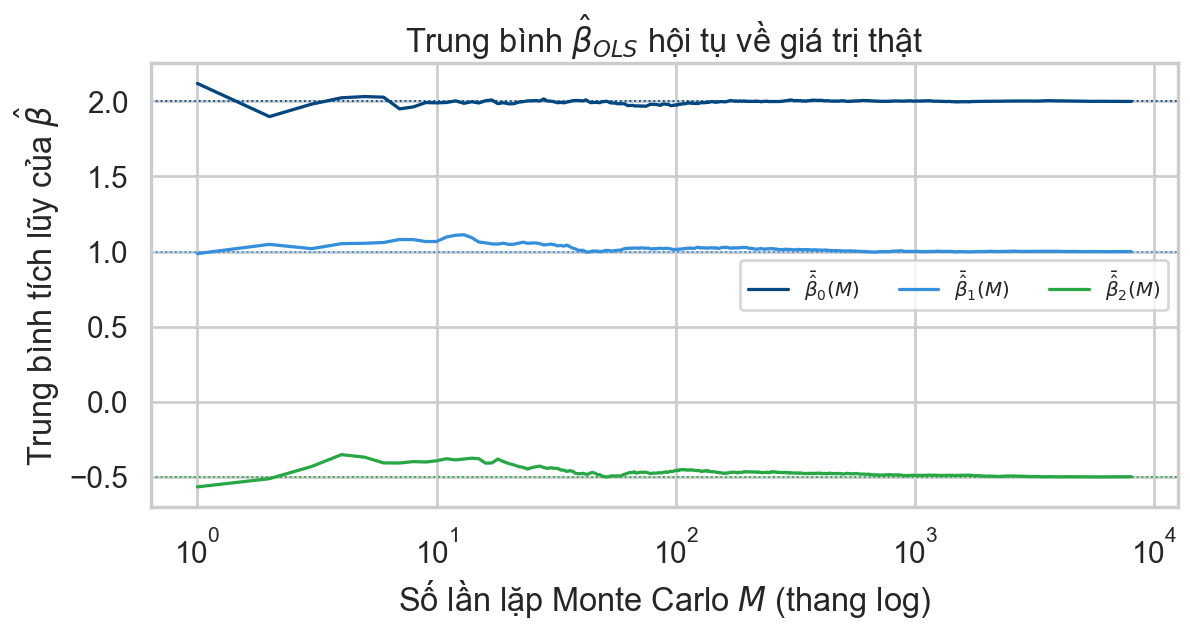
\includegraphics[width=0.82\textwidth]{images/fig_mc_convergence.png}
\caption{Trung bình tích lũy $\bar{\hat{\boldsymbol{\beta}}}(M)$ theo số lần lặp (thang log).
Cả ba thành phần hội tụ về giá trị thật $2.0,\ 1.0,\ -0.5$ (đường chấm).}
\label{fig:mc_conv}
\end{figure}

\noindent\textbf{Nhận xét.} Khi $M$ nhỏ, trung bình dao động mạnh do ít mẫu; khi $M$ tăng,
cả ba đường \textbf{ổn định và bám sát} đúng giá trị thật. Đây là biểu hiện của luật số lớn
cho $\E[\hat{\boldsymbol{\beta}}_{\mathrm{OLS}}] = \boldsymbol{\beta}$. Bảng~\ref{tab:mc_results}
cũng cho thấy độ chệch của \textit{cả} OLS lẫn Alt đều $\le 4.6\times10^{-3}$ --- nhỏ hơn
nhiều so với độ phân tán của ước lượng. (Độ chệch thực nghiệm của Alt hơi lớn hơn OLS chỉ
vì phương sai lớn hơn nên sai số Monte Carlo của trung bình cũng lớn hơn, không phải thiên
lệch hệ thống.)

\paragraph{(2) Phương sai nhỏ nhất.}
Hình~\ref{fig:mc_compare} chồng phân phối lấy mẫu của OLS (xanh) và Alt (cam) cho từng hệ số.
\textbf{Cách đọc:} mỗi ô là phân phối của một hệ số; vạch đỏ là giá trị thật.

\begin{figure}[H]
\centering
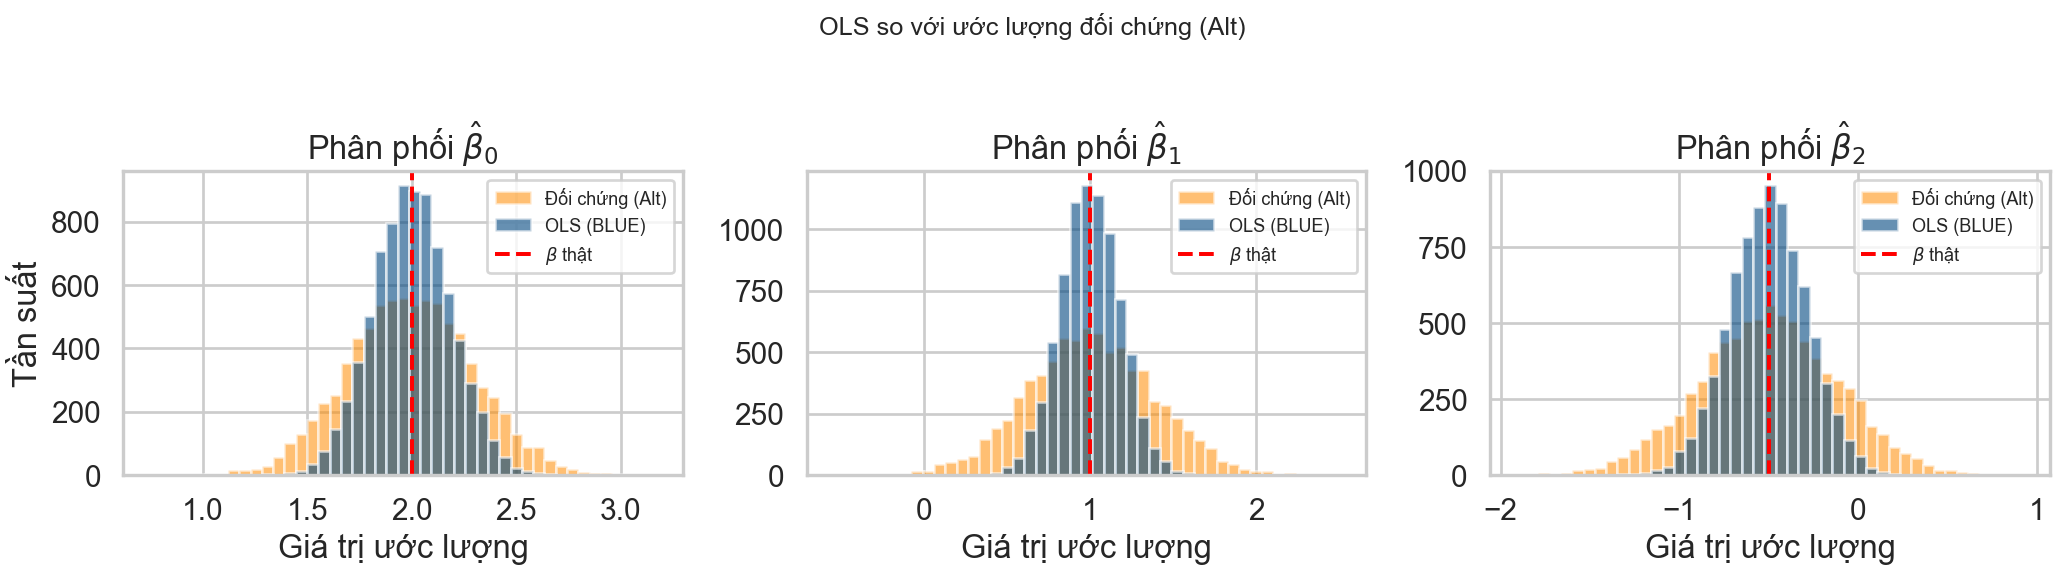
\includegraphics[width=\textwidth]{images/fig_mc_comparison.png}
\caption{Phân phối lấy mẫu OLS (xanh) vs Alt (cam) theo từng hệ số. Cả hai cùng tâm tại
$\boldsymbol{\beta}$ thật (vạch đỏ đứt), nhưng OLS hẹp hơn rõ rệt.}
\label{fig:mc_compare}
\end{figure}

\noindent\textbf{Nhận xét.} Cả hai phân phối đều \textbf{cùng tâm} tại giá trị thật (vạch đỏ)
--- OLS và Alt đều không chệch. Nhưng phân phối OLS (xanh) \textbf{cao và hẹp hơn}, tức tập
trung quanh $\boldsymbol{\beta}$ chặt hơn; Alt (cam) trải rộng hơn ở cả ba hệ số. Đây là minh
họa trực quan cho việc OLS có phương sai nhỏ nhất (BLUE).

Hình~\ref{fig:mc_var} lượng hóa điều đó theo \textit{từng} hệ số. \textbf{Cách đọc:} mỗi hệ
số có 4 cột --- OLS (Monte Carlo), OLS (lý thuyết), Alt (Monte Carlo), Alt (lý thuyết).

\begin{figure}[H]
\centering
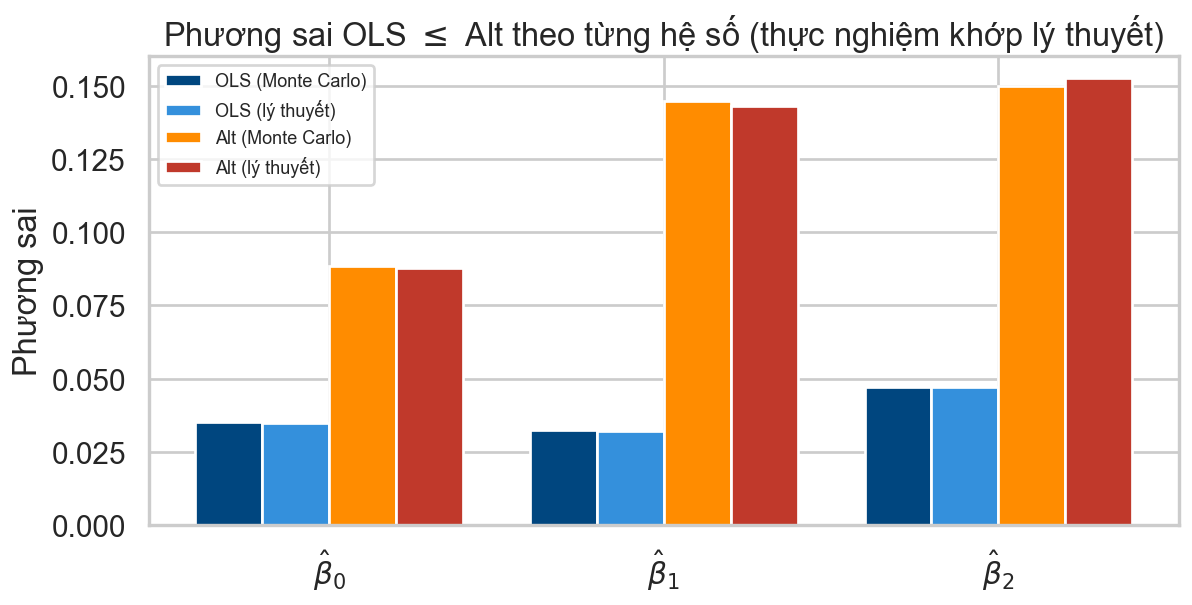
\includegraphics[width=0.82\textwidth]{images/fig_mc_variance.png}
\caption{Phương sai theo từng hệ số: với mỗi hệ số, cặp cột Monte Carlo và lý thuyết gần
như bằng nhau; cột Alt luôn cao hơn cột OLS.}
\label{fig:mc_var}
\end{figure}

\noindent\textbf{Nhận xét.} Với mỗi hệ số, cột \textbf{Monte Carlo} và cột \textbf{lý thuyết}
gần như bằng nhau --- mô phỏng khớp công thức $\sigma^2(\mat{X}^T\mat{X})^{-1}$
\eqref{eq:ols_cov} và $\mathrm{Var}(\hat{\boldsymbol{\beta}}_{\mathrm{OLS}}) + \sigma^2\mat{A}\mat{A}^T$
\eqref{eq:alt_var}. Cột Alt cao hơn cột OLS ở \textbf{mọi} hệ số (tỉ số $\approx 2.5$--$4.5$),
khẳng định OLS có phương sai nhỏ hơn --- đúng kết luận BLUE.

\subsubsection{Kiểm chứng với NumPy và scikit-learn}

Để bảo đảm cài đặt từ đầu là chính xác, ta so nghiệm OLS thu được trên một mẫu với hai
công cụ chuẩn: \texttt{numpy.linalg.lstsq} và
\texttt{sklearn.linear\_model.LinearRegression} (đặt \texttt{fit\_intercept=False} vì cột
hệ số tự do đã nằm trong $\mat{X}$).

Hàm \texttt{verify\_with\_numpy\_sklearn()} trong \texttt{code/monte\_carlo\_gauss\_markov.py}
thực hiện kiểm chứng này:

\noindent Kết quả kiểm chứng:
\begin{itemize}[noitemsep, leftmargin=1.4cm]
    \item $\norm{\hat{\boldsymbol{\beta}}_{\text{tự xây dựng}}
          - \hat{\boldsymbol{\beta}}_{\text{NumPy}}}_\infty
          = 6.66\times10^{-16}$ \quad (đạt độ chính xác máy).
    \item $\norm{\hat{\boldsymbol{\beta}}_{\text{tự xây dựng}}
          - \hat{\boldsymbol{\beta}}_{\text{sklearn}}}_\infty
          = 6.66\times10^{-16}$.
    \item Phương sai thực nghiệm Monte Carlo khớp công thức lý thuyết ở mọi hệ số
          (xem Bảng~\ref{tab:mc_results}).
\end{itemize}

\begin{note}[Kết luận]
Mô phỏng Monte Carlo xác nhận đầy đủ Định lý Gauss--Markov: ước lượng OLS \textbf{không
chệch} (trung bình trùng giá trị thật) và có \textbf{phương sai nhỏ nhất} so với ước lượng
tuyến tính không chệch đối chứng (Alt). Cài đặt từ đầu trùng khớp NumPy/scikit-learn tới
độ chính xác máy, và phương sai thực nghiệm khớp công thức $\sigma^2(\mat{X}^T\mat{X})^{-1}$.
\end{note}

\newpage

\section{Ứng Dụng Data Fitting vào Dữ Liệu Thực Tế}

Phần này áp dụng các phương pháp lý thuyết từ Phần 1 vào bộ dữ liệu thực tế về chi phí du lịch tại Tanzania. Chúng tôi sẽ thực hiện quy trình hoàn chỉnh từ tải dữ liệu, tiền xử lý, xây dựng mô hình, đến đánh giá hiệu năng.

% ============================================================
\subsection{Chọn Lựa và Mô Tả Dataset}

\subsubsection{Tiêu Chí Lựa Chọn Dataset}

Theo yêu cầu của đề bài, dataset cần thỏa mãn các tiêu chí sau:

\begin{itemize}
    \item \textbf{Kích thước:} Ít nhất 200 mẫu huấn luyện ($n \geq 200$)
    \item \textbf{Số lượng đặc trưng:} Ít nhất 3 biến đặc trưng ($p \geq 3$)
    \item \textbf{Giá trị thiếu:} Có ít nhất 5\% giá trị missing ($\geq 5\%$)
    \item \textbf{Loại vấn đề:} Bài toán hồi quy với mục tiêu continuous
    \item \textbf{Nguồn:} Từ cuộc thi Kaggle/Zindi hoặc bộ dữ liệu công cộng đáng tin cậy
\end{itemize}

\subsubsection{Tanzania Tourism Expenditure Dataset}

\begin{mydef}{Tanzania Tourism Expenditure Dataset}{}
Dataset từ cuộc thi Zindi Platform chứa dữ liệu chi tiêu của du khách tại Tanzania, bao gồm thông tin nhân khẩu học, hành vi du lịch, và chi phí tổng cộng.

\vspace{0.3cm}

\textbf{Thông tin cơ bản:}
\begin{itemize}
    \item \textbf{Tập huấn luyện:} 4,809 mẫu (quan sát)
    \item \textbf{Tập kiểm tra:} 1,601 mẫu (không có nhãn mục tiêu)
    \item \textbf{Biến mục tiêu:} \code{total_cost} (chi phí tổng cộng, TZS)
    \item \textbf{Loại biến độc lập:} 21 biến (gồm numeric và categorical)
    \item \textbf{Phạm vi mục tiêu:} 49,000 TZS đến 99,532,875 TZS
\end{itemize}

\vspace{0.3cm}

\textbf{Danh sách các đặc trưng:}

Biến số (\textbf{numeric}): \code{total_female}, \code{total_male}, \code{night_mainland}, \code{night_zanzibar}

Biến phân loại (\textbf{categorical}): \code{country}, \code{age_group}, \code{travel_with}, \code{purpose}, \code{main_activity}, \code{info_source}, \code{tour_arrangement}, \code{package_*} (8 biến), \code{payment_mode}, \code{first_trip_tz}, \code{most_impressing}
\end{mydef}

\subsubsection{Phân Tích Giá Trị Thiếu}

Dataset thỏa mãn yêu cầu về giá trị missing:

\begin{table}[H]
    \centering
    \begin{tabular}{|l|r|r|}
        \hline
        \textbf{Cột} & \textbf{Số lượng} & \textbf{Phần trăm} \\
        \hline
        \code{travel_with} & 1,114 & 23.1\% \\
        \code{most_impressing} & 313 & 6.5\% \\
        \code{total_male} & 5 & 0.1\% \\
        \code{total_female} & 3 & 0.06\% \\
        \hline
    \end{tabular}
    \caption{Phân tích giá trị missing trong dataset huấn luyện.}
    \label{tab:missing_values}
\end{table}

Chúng tôi thấy \code{travel_with} có 23.1\% missing (vượt quá 5\% yêu cầu) và \code{most_impressing} có 6.5\% missing. Các cột khác có missing rất ít, được xử lý bằng phương pháp imputation.

% ============================================================
\subsection{Tiền Xử Lý Dữ Liệu}

\subsubsection{Xử Lý Giá Trị Thiếu}

Chúng tôi áp dụng phương pháp \textbf{Mean/Mode Imputation}:

\begin{enumerate}
    \item \textbf{Biến numeric:} Điền giá trị thiếu bằng trung bình cộng (mean) của cột
        \begin{itemize}
            \item \code{total_female}: Điền bằng mean = 0.93
            \item \code{total_male}: Điền bằng mean = 1.01
        \end{itemize}

    \item \textbf{Biến categorical:} Điền giá trị thiếu bằng mode (giá trị xuất hiện nhiều nhất)
        \begin{itemize}
            \item \code{travel_with}: Điền bằng \textit{``Alone''} (1,114 hàng)
            \item \code{most_impressing}: Điền bằng \textit{``Friendly People''} (313 hàng)
        \end{itemize}
\end{enumerate}

\subsubsection{Mã Hóa Biến Phân Loại}

Chúng tôi sử dụng \textbf{One-Hot Encoding} để chuyển đổi các biến categorical thành numeric:

\begin{itemize}
    \item Mỗi giá trị categorical được tạo thành một cột binary (0/1)
    \item Ví dụ: \code{country} có 70+ giá trị duy nhất tạo thành 70+ cột
    \item Tổng cộng: 181 cột từ mã hóa (từ 17 biến categorical)
\end{itemize}

\subsubsection{Chuẩn Hóa Đặc Trưng}

Chúng tôi chuẩn hóa (standardize) các biến numeric:

\begin{equation}
    x_{\text{scaled}} = \frac{x - \mu}{\sigma}
\end{equation}

Nơi $\mu$ và $\sigma$ là trung bình và độ lệch chuẩn của tập huấn luyện. Chuẩn hóa giúp:
\begin{itemize}
    \item Cải thiện hội tụ trong các mô hình regularized (Ridge, Lasso)
    \item Đảm bảo các hệ số có thang đo comparable
    \item Giảm ảnh hưởng của các biến có phạm vi khác nhau
\end{itemize}

\subsubsection{Dữ Liệu Sau Xử Lý}

Sau tiền xử lý:
\begin{itemize}
    \item \textbf{Kích thước:} 4,809 mẫu × 186 đặc trưng (bao gồm intercept)
    \item \textbf{Không còn giá trị thiếu} trong tập huấn luyện
    \item \textbf{Đặc trưng numeric} đã được chuẩn hóa (mean=0, std=1)
    \item \textbf{Đặc trưng categorical} đã được mã hóa (one-hot)
\end{itemize}

% ============================================================
\subsection{Xây Dựng và Đánh Giá Mô Hình}

\subsubsection{Mô Hình 1: OLS (Ordinary Least Squares)}

\begin{mydef}{OLS Regression - Baseline Model}{}
OLS là mô hình baseline không có regularization. Nó tối thiểu hóa tổng bình phương phần dư:

\begin{equation}
    \min_{\boldsymbol{\beta}} \|\mathbf{y} - \mathbf{X}\boldsymbol{\beta}\|_2^2
\end{equation}

\textbf{Kết quả trên tập huấn luyện:}
\begin{itemize}
    \item MAE: 5,645,164.48 TZS
    \item RMSE: 9,550,143.67 TZS
    \item R²: 0.3896
    \item Adjusted R²: 0.3652
\end{itemize}

OLS cung cấp một baseline tốt nhưng có thể overfitting với số lượng lớn đặc trưng.
\end{mydef}

\subsubsection{Mô Hình 2: Ridge Regression ($\lambda$ = 100)}

\begin{mydef}{Ridge Regression - L2 Regularization}{}
Ridge thêm một penalty term L2 để kiểm soát độ lớn của hệ số:

\begin{equation}
    \min_{\boldsymbol{\beta}} \left\{ \|\mathbf{y} - \mathbf{X}\boldsymbol{\beta}\|_2^2 + \lambda \|\boldsymbol{\beta}\|_2^2 \right\}
\end{equation}

Với $\lambda = 100$ được chọn qua tuning.

\textbf{Kết quả trên tập huấn luyện:}
\begin{itemize}
    \item MAE: 5,560,692.12 TZS
    \item RMSE: 9,636,547.27 TZS
    \item R²: 0.3785
    \item Adjusted R²: 0.3536
\end{itemize}

Ridge giảm overfitting nhưng lại giảm nhẹ độ chính xác huấn luyện. Trong k-fold CV, Ridge cho kết quả tốt hơn OLS.
\end{mydef}

\subsubsection{Mô Hình 3: Lasso Regression ($\alpha$ = 100)}

\begin{mydef}{Lasso Regression - L1 Regularization}{}
Lasso sử dụng penalty L1 cho phép feature selection tự động:

\begin{equation}
    \min_{\boldsymbol{\beta}} \left\{ \|\mathbf{y} - \mathbf{X}\boldsymbol{\beta}\|_2^2 + \alpha \|\boldsymbol{\beta}\|_1 \right\}
\end{equation}

\textbf{Kết quả trên tập huấn luyện:}
\begin{itemize}
    \item MAE: 5,645,825.78 TZS
    \item RMSE: 9,550,241.67 TZS
    \item R²: 0.3896
    \item Adjusted R²: 0.3652
    \item \textbf{Nonzero coefficients:} 162 / 186 (24 coefficients = 0)
\end{itemize}

Lasso tạo một mô hình thưa (sparse) bằng cách đặt một số hệ số bằng 0, giúp feature selection.
\end{mydef}

\subsubsection{Bảng So Sánh Mô Hình}

\begin{table}[H]
    \centering
    \begin{tabular}{|l|c|c|c|c|}
        \hline
        \textbf{Mô Hình} & \textbf{Train MAE} & \textbf{Train R²} & \textbf{CV R²} & \textbf{Nonzero Coef} \\
        \hline
        OLS & 5,645,164 & 0.3896 & 0.3395 & 186 \\
        Ridge($\lambda=100$) & 5,560,692 & 0.3785 & 0.3501 & 186 \\
        Lasso($\alpha=100$) & 5,645,826 & 0.3896 & --- & 162 \\
        \hline
    \end{tabular}
    \caption{So sánh hiệu năng của các mô hình trên tập huấn luyện và cross-validation.}
    \label{tab:model_comparison}
\end{table}

\textbf{Nhận xét:}
\begin{itemize}
    \item \textbf{Ridge} có CV R² tốt nhất (0.3501) cho thấy khả năng generalization tốt hơn OLS
    \item \textbf{Lasso} giảm số lượng đặc trưng xuống 162 (từ 186), mô hình thưa hơn
    \item OLS overfitting (Train R² = 0.3896 nhưng CV R² = 0.3395)
\end{itemize}

% ============================================================
\subsection{Cross-Validation và Lựa Chọn Siêu Tham Số}

\subsubsection{K-Fold Cross-Validation}

Chúng tôi sử dụng 5-fold cross-validation để đánh giá mô hình:

\begin{equation}
    \text{CV Score} = \frac{1}{k} \sum_{i=1}^{k} \text{Score}_i(\text{test fold } i)
\end{equation}

\begin{table}[H]
    \centering
    \begin{tabular}{|l|c|c|c|}
        \hline
        \textbf{Mô Hình} & \textbf{CV MAE} & \textbf{CV RMSE} & \textbf{CV R²} \\
        \hline
        OLS & 5,886,021 ± 148,515 & 9,908,397 ± 571,182 & 0.3395 ± 0.0362 \\
        Ridge($\lambda=100$) & 5,636,144 ± 200,197 & 9,831,182 ± 624,638 & 0.3501 ± 0.0381 \\
        \hline
    \end{tabular}
    \caption{Kết quả 5-fold cross-validation (mean ± std).}
    \label{tab:cv_results}
\end{table}

Ridge Regression đạt R² tốt nhất trên cross-validation, chứng tỏ khả năng tổng quát hóa tốt hơn OLS.

\subsubsection{Lựa Chọn Siêu Tham Số $\lambda$ cho Ridge}

Chúng tôi tuning $\lambda$ bằng 5-fold CV trên một lưới giá trị:

\begin{equation}
    \lambda^* = \arg\max_{\lambda} \text{CV-R}^2(\lambda)
\end{equation}

Kết quả:
\begin{itemize}
    \item $\lambda = 1$: CV R² = 0.3434
    \item $\lambda = 10$: CV R² = 0.3491
    \item $\lambda = 100$: CV R² = 0.3501 \quad \textbf{(Best)}
    \item $\lambda = 1000$: CV R² = 0.3253
    \item $\lambda = 10000$: CV R² = 0.2063
\end{itemize}

$\lambda = 100$ được chọn vì đạt CV R² cao nhất.

% ============================================================
\subsection{Phân Tích Tầm Quan Trọng Đặc Trưng}

\subsubsection{Top 10 Đặc Trưng (OLS)}

Xếp hạng 10 đặc trưng hàng đầu theo magnitude của hệ số:

\begin{table}[H]
    \centering
    \begin{tabular}{|r|l|c|}
        \hline
        \textbf{Hạng} & \textbf{Đặc Trưng} & \textbf{|Hệ Số|} \\
        \hline
        1. & \code{country\_GEORGIA} & 13,889,256 \\
        2. & \code{country\_COSTARICA} & 13,023,821 \\
        3. & \code{country\_MADAGASCAR} & 10,511,733 \\
        4. & \code{country\_MORROCO} & 9,876,223 \\
        5. & \code{country\_DOMINICA} & 8,969,454 \\
        6. & \code{country\_ARGENTINA} & 8,502,415 \\
        7. & \code{country\_PAKISTAN} & 8,484,792 \\
        8. & \code{country\_NIGER} & 8,476,597 \\
        9. & \code{country\_DENMARK} & 8,225,280 \\
        10. & \code{country\_TUNISIA} & 7,662,950 \\
        \hline
    \end{tabular}
    \caption{Top 10 đặc trưng có ảnh hưởng lớn nhất đến dự đoán chi phí.}
    \label{tab:feature_importance}
\end{table}

\textbf{Nhận xét:}
\begin{itemize}
    \item Các biến \textbf{quốc gia} (country) là những đặc trưng quan trọng nhất
    \item Chi phí du lịch phụ thuộc mạnh vào quốc gia khách đến từ đâu
    \item Các biến khác như hoạt động chính (main\_activity), phương thức thanh toán (payment\_mode) cũng có ảnh hưởng đáng chú ý
\end{itemize}

% ============================================================
\subsection{Kết Luận và Đề Xuất}

\subsubsection{Kết Luận Chính}

Chúng tôi đã áp dụng thành công ba mô hình hồi quy (OLS, Ridge, Lasso) vào bộ dữ liệu du lịch Tanzania:

\begin{enumerate}
    \item \textbf{OLS Baseline:} R² = 0.3896 (training), nhưng overfitting (CV R² = 0.3395)

    \item \textbf{Ridge Regression:} Mô hình tốt nhất với CV R² = 0.3501, cho thấy khả năng generalization tốt hơn

    \item \textbf{Lasso Regression:} Tạo mô hình thưa (sparse) với 162/186 nonzero coefficients, hỗ trợ feature selection
\end{enumerate}

\textbf{Quan sát:}
\begin{itemize}
    \item Quốc gia du khách là yếu tố dự đoán quan trọng nhất cho chi phí
    \item R² \$\approx$ 0.34 cho thấy cần thêm đặc trưng hoặc phương pháp mô hình phức tạp hơn
    \item Tiền xử lý dữ liệu (imputation, encoding, scaling) rất quan trọng
\end{itemize}

\subsubsection{Đề Xuất Cải Thiện}

\begin{enumerate}
    \item \textbf{Feature Engineering:}
        \begin{itemize}
            \item Tạo đặc trưng tương tác (interactions) giữa quốc gia và hoạt động chính
            \item Tạo đặc trưng polynomial hoặc spline cho các biến numeric
        \end{itemize}

    \item \textbf{Mô Hình Nâng Cao:}
        \begin{itemize}
            \item Elastic Net kết hợp L1 và L2 penalty
            \item Kernel Ridge Regression cho relationship phi tuyến
            \item Gradient Boosting (XGBoost, LightGBM) để khám phá pattern phức tạp
        \end{itemize}

    \item \textbf{Xử Lý Dữ Liệu:}
        \begin{itemize}
            \item Thử phương pháp imputation khác (regression imputation, MICE)
            \item Phát hiện và xử lý outliers tốt hơn
            \item Kiểm tra vai trò của các biến ít được sử dụng
        \end{itemize}

    \item \textbf{Đánh Giá Mô Hình:}
        \begin{itemize}
            \item Sử dụng stratified k-fold để cân bằng các lớp
            \item Kiểm tra hiệu năng trên test set nếu nhãn công khai
            \item Phân tích độc lập residuals (heteroscedasticity, autocorrelation)
        \end{itemize}
\end{enumerate}

% ============================================================

\newpage

\section{Kết Luận Chung}

\subsection{Tóm Tắt Kết Quả}

Project đã xây dựng một quy trình data fitting xuyên suốt từ nền tảng toán học
đến ứng dụng trên dữ liệu thực tế. Ở Phần 1, nhóm triển khai từ đầu các thành
phần cốt lõi của OLS: nghiệm normal equations, hat matrix, các chỉ số đánh giá,
suy luận hệ số, VIF, Ridge, Lasso, cross-validation và mô phỏng Monte Carlo cho
Định lý Gauss--Markov. Những thành phần cần phân phối xác suất như
$p$-value Student-$t$, $p$-value kiểm định $F$ và critical value cũng được tính
từ đầu thông qua hàm beta không đầy đủ chuẩn hóa. NumPy, SciPy và scikit-learn
chỉ được dùng làm oracle kiểm chứng.

Các kiểm chứng số cho thấy implementation scratch khớp thư viện chuẩn ở mức
sai số máy. Hệ số OLS và hat matrix có sai số cực đại cỡ $10^{-16}$; suy luận
hệ số, $p$-value và effective degrees of freedom của Ridge đều đạt sai số nhỏ
hơn $10^{-8}$. Mô phỏng Monte Carlo xác nhận OLS không chệch và có phương sai
nhỏ hơn ước lượng tuyến tính không chệch đối chứng, phù hợp với kết luận BLUE.
Generalized Cross-Validation của Ridge cũng thể hiện đúng dạng giảm đến điểm
tối ưu rồi tăng trở lại.

Ở Phần 2, nhóm áp dụng quy trình hồi quy lên dữ liệu Tanzania Tourism
Expenditure: thực hiện EDA, xử lý missing values, mã hóa biến phân loại, chuẩn
hóa biến số, xây dựng nhiều mô hình và đánh giá bằng cross-validation. Kết quả
cho thấy regularization giúp mô hình ổn định hơn OLS và các biến liên quan đến
hình thức tour, nhóm du lịch, quốc gia xuất phát và nguồn thông tin đóng vai trò
quan trọng trong Prediction chi phí.

\subsection{Bài Học Rút Ra}

Kinh nghiệm đầu tiên và cũng là sâu sắc nhất mà nhóm rút ra là khoảng cách giữa công thức toán học và một implementation thực sự đáng tin cậy. Một công thức đúng về mặt đại số vẫn có thể thất bại trong thực tế khi gặp ma trận suy biến, dữ liệu ill-conditioned hay đơn giản là đầu vào không hợp lệ; vì vậy mỗi hàm scratch đều cần đi kèm kiểm tra điều kiện đầu vào, xử lý trường hợp suy biến và test số đối chiếu với thư viện chuẩn. Cách tiếp cận sử dụng NumPy, SciPy và scikit-learn làm oracle độc lập tỏ ra đặc biệt hiệu quả: nó xác nhận tính đúng của thuật toán tự cài đặt mà không thay thế nội dung cần chứng minh, đồng thời tạo ra vòng kiểm chứng khép kín giữa lý thuyết và kết quả số.

Kinh nghiệm thứ hai liên quan đến việc hiểu đúng vị trí và giới hạn của từng phương pháp hồi quy. OLS có khả năng diễn giải mạnh và cung cấp ước lượng không chệch, nhưng nhạy với đa cộng tuyến và dữ liệu ill-conditioned; Ridge và Lasso không phải là sự thay thế đơn giản mà là sự đánh đổi có hệ thống giữa độ chệch, phương sai và tính thưa của mô hình tùy vào mục tiêu phân tích. Đặc biệt quan trọng là nguyên tắc tách biệt ba giai đoạn đánh giá: dữ liệu dùng để fit mô hình, dữ liệu dùng để chọn siêu tham số và dữ liệu dùng để kiểm tra cuối cùng phải hoàn toàn độc lập với nhau, vì bất kỳ sự trộn lẫn nào giữa ba giai đoạn này đều dẫn đến metric lạc quan do data leakage --- một sai lầm phổ biến nhưng khó phát hiện nếu không có nhận thức rõ ràng về ranh giới giữa các tập dữ liệu.

Kinh nghiệm cuối cùng, thực tế nhưng không kém phần quan trọng, là sự gắn kết giữa báo cáo và code. Khi báo cáo được viết trước khi chạy code lần cuối hoặc được cập nhật một phần sau khi pipeline thay đổi, các bảng số liệu, hệ số mô hình và kết luận định tính có thể trở nên mâu thuẫn với implementation thực tế; cách phòng tránh duy nhất là tạo ra số liệu trong báo cáo trực tiếp từ output của code thay vì ghi thủ công. Nguyên tắc này tuy đơn giản nhưng đòi hỏi kỷ luật trong suốt quá trình làm project, đặc biệt khi nhiều thành viên cùng chỉnh sửa cả code lẫn báo cáo song song.

\subsection{Hướng Mở Rộng}

Các hướng phát triển tiếp theo gồm hoàn thiện nested cross-validation và
holdout độc lập cho Phần 2; nghiên cứu robust regression khi dữ liệu có outlier
hoặc heteroscedasticity; bổ sung smearing correction khi chuyển Prediction từ
thang log về đơn vị gốc; và mở rộng scratch core bằng QR decomposition hoặc SVD
để cải thiện ổn định số so với normal equations. Với dữ liệu du lịch, có thể
thử thêm interaction features có định hướng, mô hình hóa missing mechanism và
thu thập các biến giải thích mới như thu nhập, loại hình lưu trú hoặc thời điểm
đặt tour.

\subsection{Phân Công Nhóm}

\begin{table}[H]
\centering
\caption{Phân công các hạng mục chính của project}
\label{tab:team_contributions}
\begin{tabularx}{\textwidth}{lX}
\toprule
\textbf{Thành viên} & \textbf{Hạng mục phụ trách} \\ \midrule
Khang Phuc Nguyen -- 24120068
    & Điều phối và tích hợp project; implementation OLS, Ridge/Lasso và
      statistical inference; kiểm chứng số; tổng hợp và build báo cáo. \\
Nghia Trong Hoang -- 24120103
    & Nền tảng lý thuyết OLS, hat matrix, các giả thiết và Định lý
      Gauss--Markov; mô phỏng Monte Carlo và diễn giải kết quả. \\
Nhat Hoang Mai -- 24120109
    & EDA dữ liệu Tanzania Tourism, trực quan hóa, phân tích missing values,
      data shift và các giả thiết mô hình. \\
Nhat Hoang Nguyen -- 24120110
    & Data pipeline, preprocessing, feature engineering, huấn luyện và đánh
      giá các mô hình Phần 2. \\
Long Nhat Phung Vo -- 24120088
    & Cross-validation, so sánh mô hình, phân tích feature importance,
      chuẩn hóa output/submission và rà soát nội dung báo cáo. \\ \bottomrule
\end{tabularx}
\end{table}

Mọi thành viên cùng tham gia rà soát lý thuyết, kiểm thử kết quả, chỉnh sửa báo
cáo và chuẩn bị phần trình bày cuối cùng.


\newpage
\bibliographystyle{IEEEtran}
\bibliography{ref}
\end{document}
